% Options for packages loaded elsewhere
\PassOptionsToPackage{unicode}{hyperref}
\PassOptionsToPackage{hyphens}{url}
%
\documentclass[
  oneside]{book}
\usepackage{lmodern}
\usepackage{amsmath}
\usepackage{ifxetex,ifluatex}
\ifnum 0\ifxetex 1\fi\ifluatex 1\fi=0 % if pdftex
  \usepackage[T1]{fontenc}
  \usepackage[utf8]{inputenc}
  \usepackage{textcomp} % provide euro and other symbols
  \usepackage{amssymb}
\else % if luatex or xetex
  \usepackage{unicode-math}
  \defaultfontfeatures{Scale=MatchLowercase}
  \defaultfontfeatures[\rmfamily]{Ligatures=TeX,Scale=1}
\fi
% Use upquote if available, for straight quotes in verbatim environments
\IfFileExists{upquote.sty}{\usepackage{upquote}}{}
\IfFileExists{microtype.sty}{% use microtype if available
  \usepackage[]{microtype}
  \UseMicrotypeSet[protrusion]{basicmath} % disable protrusion for tt fonts
}{}
\makeatletter
\@ifundefined{KOMAClassName}{% if non-KOMA class
  \IfFileExists{parskip.sty}{%
    \usepackage{parskip}
  }{% else
    \setlength{\parindent}{0pt}
    \setlength{\parskip}{6pt plus 2pt minus 1pt}}
}{% if KOMA class
  \KOMAoptions{parskip=half}}
\makeatother
\usepackage{xcolor}
\IfFileExists{xurl.sty}{\usepackage{xurl}}{} % add URL line breaks if available
\IfFileExists{bookmark.sty}{\usepackage{bookmark}}{\usepackage{hyperref}}
\hypersetup{
  pdftitle={Vegetation modelling},
  pdfauthor={Hans Verbeeck, Elizabeth Kearsley, Félicien Meunier, Marc Peaucelle},
  hidelinks,
  pdfcreator={LaTeX via pandoc}}
\urlstyle{same} % disable monospaced font for URLs
\usepackage[left=3cm,right=3cm,top=2cm,bottom=2cm]{geometry}
\usepackage{color}
\usepackage{fancyvrb}
\newcommand{\VerbBar}{|}
\newcommand{\VERB}{\Verb[commandchars=\\\{\}]}
\DefineVerbatimEnvironment{Highlighting}{Verbatim}{commandchars=\\\{\}}
% Add ',fontsize=\small' for more characters per line
\usepackage{framed}
\definecolor{shadecolor}{RGB}{248,248,248}
\newenvironment{Shaded}{\begin{snugshade}}{\end{snugshade}}
\newcommand{\AlertTok}[1]{\textcolor[rgb]{0.94,0.16,0.16}{#1}}
\newcommand{\AnnotationTok}[1]{\textcolor[rgb]{0.56,0.35,0.01}{\textbf{\textit{#1}}}}
\newcommand{\AttributeTok}[1]{\textcolor[rgb]{0.77,0.63,0.00}{#1}}
\newcommand{\BaseNTok}[1]{\textcolor[rgb]{0.00,0.00,0.81}{#1}}
\newcommand{\BuiltInTok}[1]{#1}
\newcommand{\CharTok}[1]{\textcolor[rgb]{0.31,0.60,0.02}{#1}}
\newcommand{\CommentTok}[1]{\textcolor[rgb]{0.56,0.35,0.01}{\textit{#1}}}
\newcommand{\CommentVarTok}[1]{\textcolor[rgb]{0.56,0.35,0.01}{\textbf{\textit{#1}}}}
\newcommand{\ConstantTok}[1]{\textcolor[rgb]{0.00,0.00,0.00}{#1}}
\newcommand{\ControlFlowTok}[1]{\textcolor[rgb]{0.13,0.29,0.53}{\textbf{#1}}}
\newcommand{\DataTypeTok}[1]{\textcolor[rgb]{0.13,0.29,0.53}{#1}}
\newcommand{\DecValTok}[1]{\textcolor[rgb]{0.00,0.00,0.81}{#1}}
\newcommand{\DocumentationTok}[1]{\textcolor[rgb]{0.56,0.35,0.01}{\textbf{\textit{#1}}}}
\newcommand{\ErrorTok}[1]{\textcolor[rgb]{0.64,0.00,0.00}{\textbf{#1}}}
\newcommand{\ExtensionTok}[1]{#1}
\newcommand{\FloatTok}[1]{\textcolor[rgb]{0.00,0.00,0.81}{#1}}
\newcommand{\FunctionTok}[1]{\textcolor[rgb]{0.00,0.00,0.00}{#1}}
\newcommand{\ImportTok}[1]{#1}
\newcommand{\InformationTok}[1]{\textcolor[rgb]{0.56,0.35,0.01}{\textbf{\textit{#1}}}}
\newcommand{\KeywordTok}[1]{\textcolor[rgb]{0.13,0.29,0.53}{\textbf{#1}}}
\newcommand{\NormalTok}[1]{#1}
\newcommand{\OperatorTok}[1]{\textcolor[rgb]{0.81,0.36,0.00}{\textbf{#1}}}
\newcommand{\OtherTok}[1]{\textcolor[rgb]{0.56,0.35,0.01}{#1}}
\newcommand{\PreprocessorTok}[1]{\textcolor[rgb]{0.56,0.35,0.01}{\textit{#1}}}
\newcommand{\RegionMarkerTok}[1]{#1}
\newcommand{\SpecialCharTok}[1]{\textcolor[rgb]{0.00,0.00,0.00}{#1}}
\newcommand{\SpecialStringTok}[1]{\textcolor[rgb]{0.31,0.60,0.02}{#1}}
\newcommand{\StringTok}[1]{\textcolor[rgb]{0.31,0.60,0.02}{#1}}
\newcommand{\VariableTok}[1]{\textcolor[rgb]{0.00,0.00,0.00}{#1}}
\newcommand{\VerbatimStringTok}[1]{\textcolor[rgb]{0.31,0.60,0.02}{#1}}
\newcommand{\WarningTok}[1]{\textcolor[rgb]{0.56,0.35,0.01}{\textbf{\textit{#1}}}}
\usepackage{longtable,booktabs}
\usepackage{calc} % for calculating minipage widths
% Correct order of tables after \paragraph or \subparagraph
\usepackage{etoolbox}
\makeatletter
\patchcmd\longtable{\par}{\if@noskipsec\mbox{}\fi\par}{}{}
\makeatother
% Allow footnotes in longtable head/foot
\IfFileExists{footnotehyper.sty}{\usepackage{footnotehyper}}{\usepackage{footnote}}
\makesavenoteenv{longtable}
\usepackage{graphicx}
\makeatletter
\def\maxwidth{\ifdim\Gin@nat@width>\linewidth\linewidth\else\Gin@nat@width\fi}
\def\maxheight{\ifdim\Gin@nat@height>\textheight\textheight\else\Gin@nat@height\fi}
\makeatother
% Scale images if necessary, so that they will not overflow the page
% margins by default, and it is still possible to overwrite the defaults
% using explicit options in \includegraphics[width, height, ...]{}
\setkeys{Gin}{width=\maxwidth,height=\maxheight,keepaspectratio}
% Set default figure placement to htbp
\makeatletter
\def\fps@figure{htbp}
\makeatother
\setlength{\emergencystretch}{3em} % prevent overfull lines
\providecommand{\tightlist}{%
  \setlength{\itemsep}{0pt}\setlength{\parskip}{0pt}}
\setcounter{secnumdepth}{5}
\usepackage{booktabs}
\usepackage{fancyhdr}

\AtBeginDocument{\let\maketitle\relax} % To relax 

% Remove page number on page parts
\usepackage{etoolbox}
\patchcmd{\part}{\thispagestyle{plain}}{\thispagestyle{empty}}{}{}

% Header and font 
\usepackage{fancyhdr}
\pagestyle{fancy}
\fancyhf{} % sets both header and footer to nothing
\renewcommand{\headrulewidth}{0pt} % Remove line

\fancyhead[L,C,R]{} % Empty header
\fancyfoot[C]{\thepage} % Footer, center, page number
\fancyfoot[L,R]{} % Empty footer on left and right
\ifluatex
  \usepackage{selnolig}  % disable illegal ligatures
\fi
\usepackage[]{natbib}
\bibliographystyle{apalike}

\title{Vegetation modelling}
\author{Hans Verbeeck, Elizabeth Kearsley, Félicien Meunier, Marc Peaucelle}
\date{2021-02-05}

\begin{document}
\maketitle

\newcommand{\plogo}{\fbox{$\mathcal{PL}$}} % Generic dummy publisher logo
\frontmatter


\begin{titlepage} % Suppresses headers and footers on the title page

	\centering % Centre everything on the title page
	
	\scshape % Use small caps for all text on the title page
	
	\vspace*{\baselineskip} % White space at the top of the page
	
	%------------------------------------------------
	%	Title
	%------------------------------------------------
	
	\vspace{12\baselineskip}
	
	\rule{\textwidth}{1.6pt}\vspace*{-\baselineskip}\vspace*{2pt} % Thick horizontal rule
	\rule{\textwidth}{0.4pt} % Thin horizontal rule
	
	\vspace{0.75\baselineskip} % Whitespace above the title
	
	{\LARGE Vegetation modelling\\} % Title
	
	\vspace{0.75\baselineskip} % Whitespace below the title
	
	\rule{\textwidth}{0.4pt}\vspace*{-\baselineskip}\vspace{3.2pt} % Thin horizontal rule
	\rule{\textwidth}{1.6pt} % Thick horizontal rule
	
	\vspace{2\baselineskip} % Whitespace after the title block
	
	%------------------------------------------------
	%	Subtitle
	%------------------------------------------------
	
	Syllabus % Subtitle or further description
	
	\vspace*{3\baselineskip} % Whitespace under the subtitle
	
	%------------------------------------------------
	%	Editor(s)
	%------------------------------------------------
	
	Written By
	
	\vspace{0.5\baselineskip} % Whitespace before the editors
	
	{\scshape Hans Verbeeck, Felicien Meunier, Marc Peaucelle \\} % Editor list
	
	\vspace{0.5\baselineskip} % Whitespace below the editor list
	
	\textit{Ghent University \\} % Editor affiliation
	
	\vfill % Whitespace between editor names and publisher logo
	
	%------------------------------------------------
	%	Publisher
	%------------------------------------------------
	
	%\plogo % Publisher logo
	
	
\includegraphics[width = 50mm]{figures/UGhent2.png}
	
	\vspace{0.3\baselineskip} % Whitespace under the publisher logo
	
	2021 % Publication year
	
	%{\large publisher} % Publisher

\end{titlepage}



{
\setcounter{tocdepth}{1}
\tableofcontents
}
\mainmatter

\hypertarget{intro}{%
\chapter{Introduction}\label{intro}}

\hypertarget{soil-plant-atmosphere-continuum-the-central-role-of-vegetation-in-the-earth-system}{%
\section{Soil-plant-atmosphere continuum: the central role of vegetation in the earth system}\label{soil-plant-atmosphere-continuum-the-central-role-of-vegetation-in-the-earth-system}}

\begin{figure}

{\centering 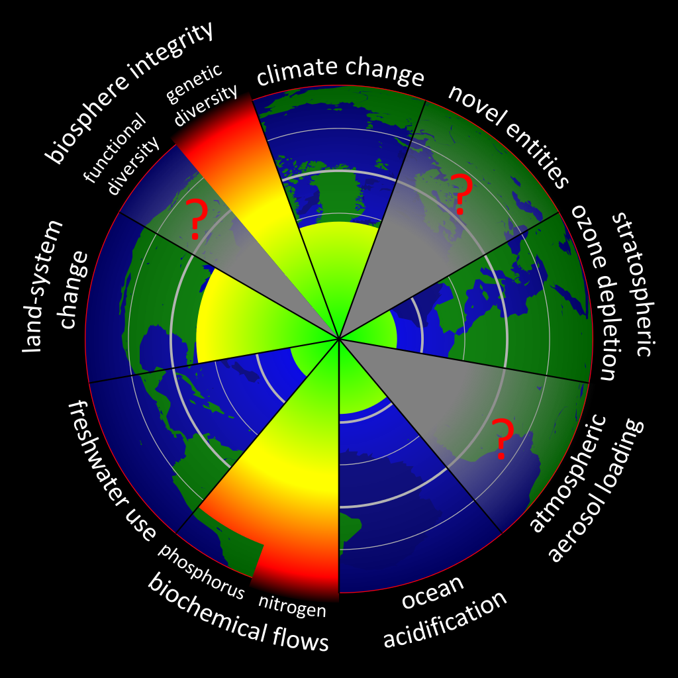
\includegraphics[width=0.8\linewidth]{figures/chap1/planetary_boundaries} 

}

\caption{The planetary boundaries (www.stockholmresilience.org)}\label{fig:f1}
\end{figure}

\begin{figure}

{\centering 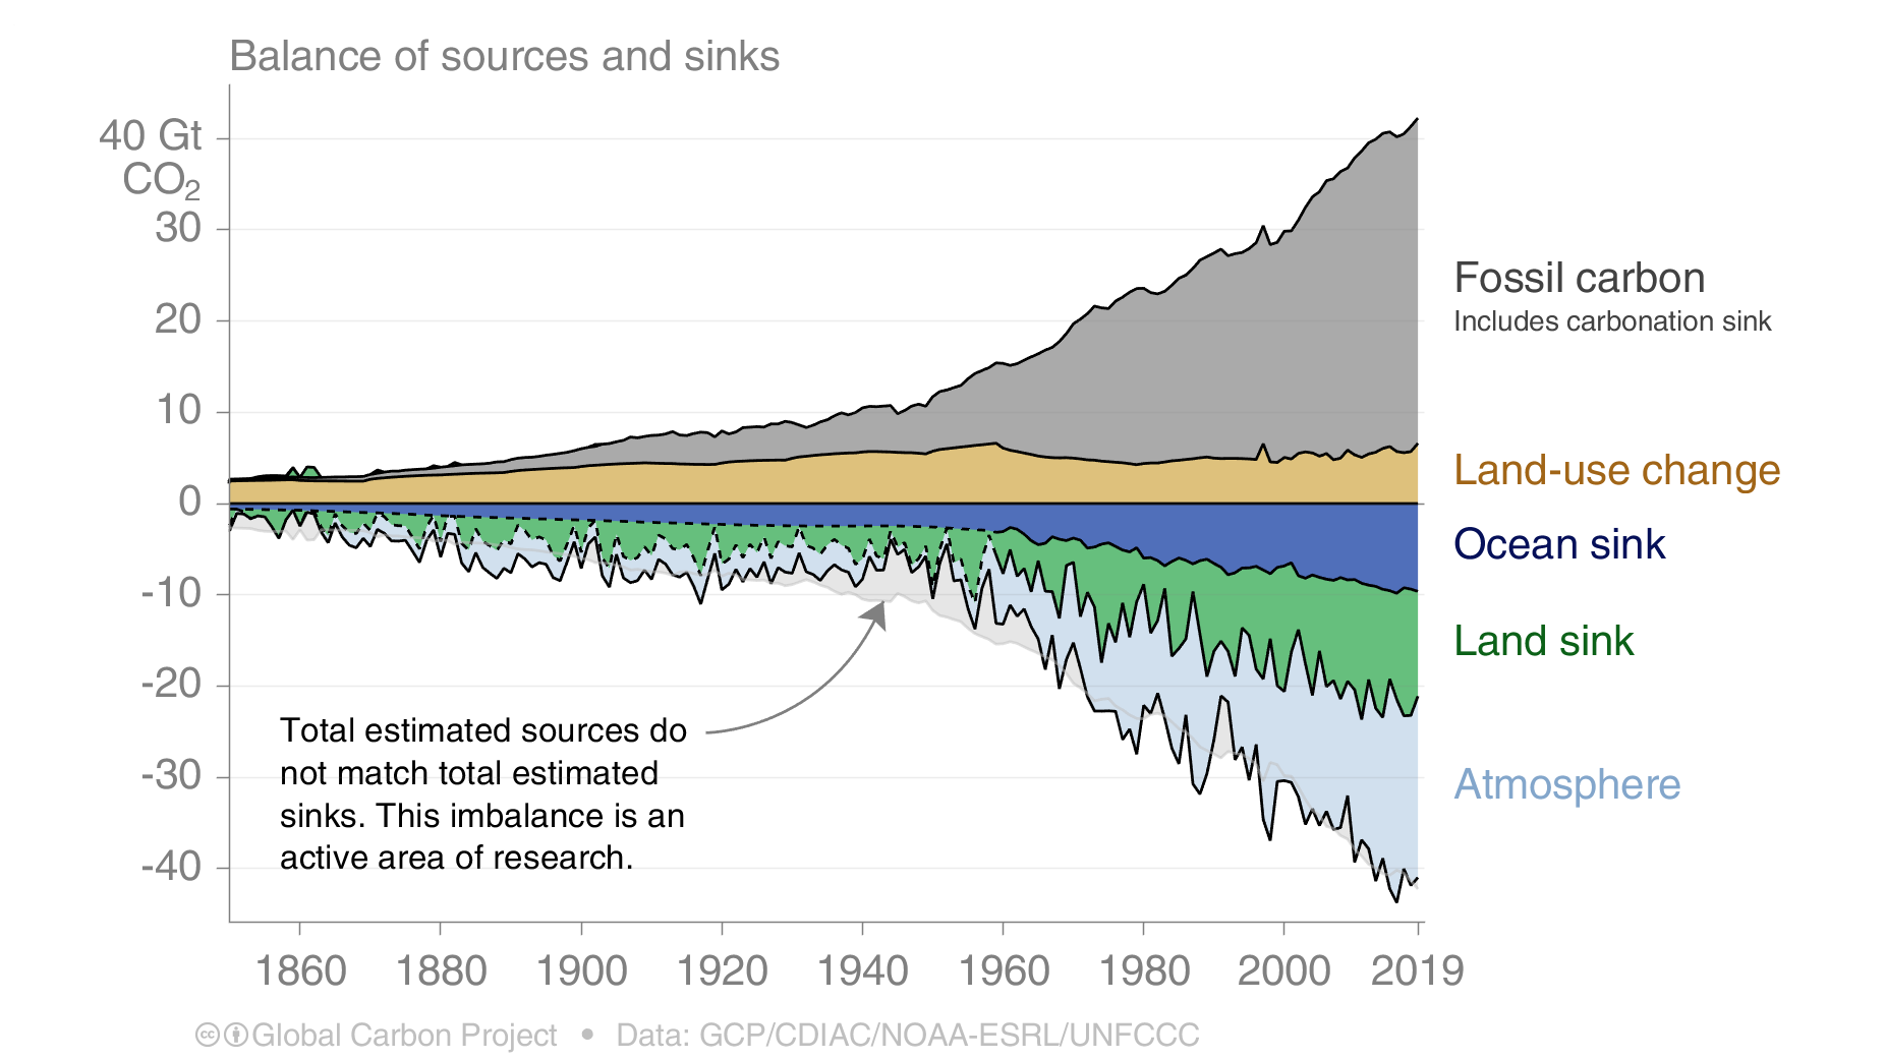
\includegraphics[width=0.8\linewidth]{figures/chap1/carbon_budget} 

}

\caption{The global carbon budget (www.globalcarbonproject.org)}\label{fig:f2}
\end{figure}

\begin{figure}

{\centering 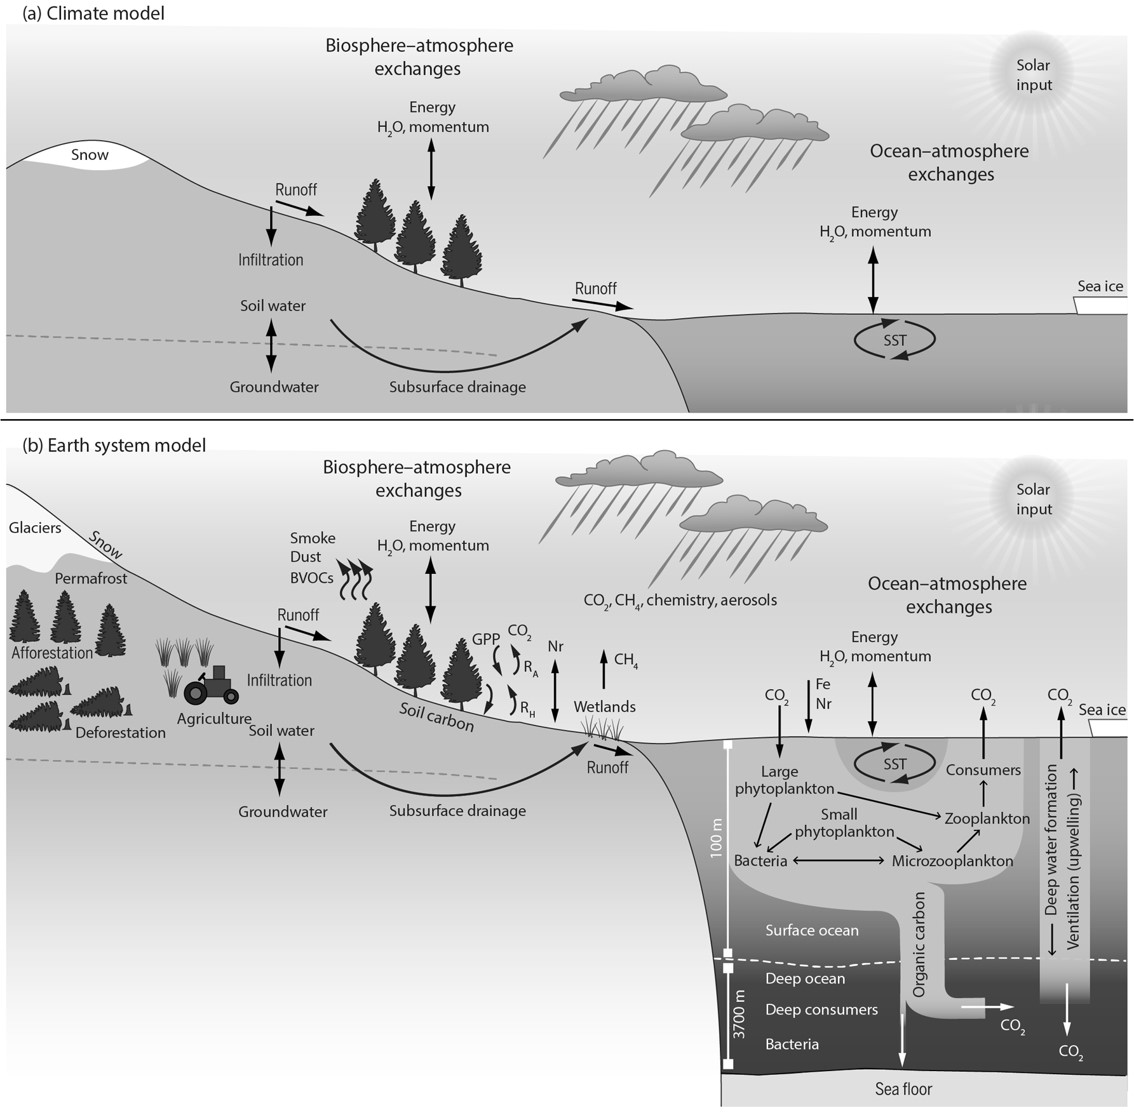
\includegraphics[width=0.8\linewidth]{figures/chap1/GCM_ESM} 

}

\caption{Scientific scope of (a) climate models and (b) earth system models. (Bonan 2019)}\label{fig:f3}
\end{figure}

\begin{figure}

{\centering 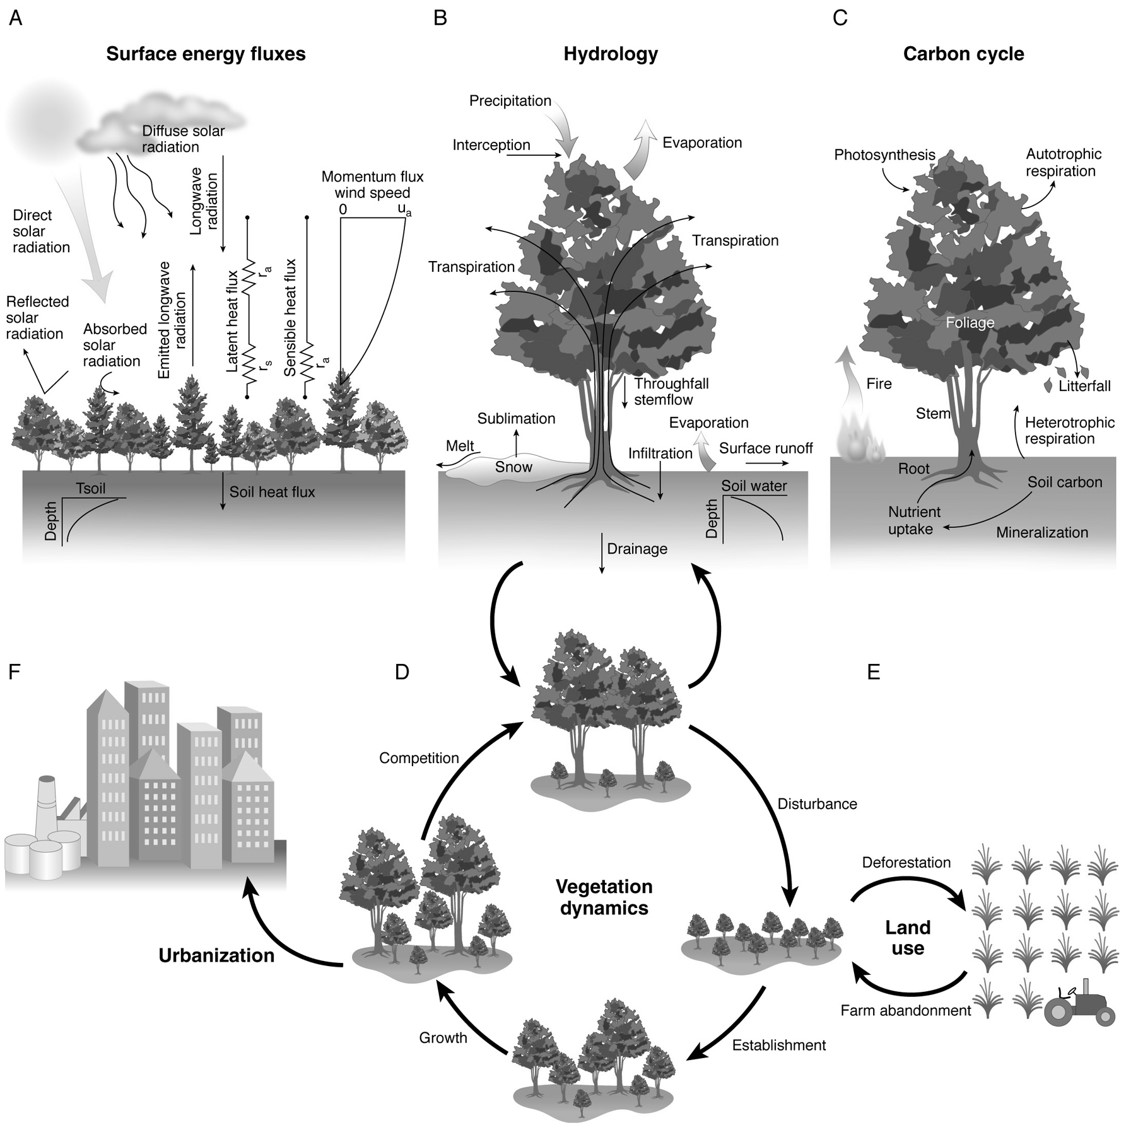
\includegraphics[width=0.8\linewidth]{figures/chap1/cycles_bonan} 

}

\caption{Scientific scope of terrestrial biosphere model. (Bonan 2019)}\label{fig:f4}
\end{figure}

\begin{itemize}
\tightlist
\item
  Global change context
\item
  Terrestrial ecosystems are central to solving the environmental and socioeconomic threats posed by changes in climate, atmospheric composition, and air quality; land use and land-cover change; habitat loss, species extinction, and invasive species; appropriation of freshwater, net primary production, and other ecosystems goods and services for human uses; and anthropogenic addition of reactive nitrogen. (Bonan)
\item
  Earth System Models and climate models (Fig 1.1 Bonan). In climate models vegetation is just representing physical fluxes, in ESM vegetation is representing biogeochemical cycles, biogeography, and dynamic vegetation -- typically the realm of ecosystem models
\item
  Land component continuum of terrestrial ecosystem models (vegetation models) (Fig 1.7)
\end{itemize}

\hypertarget{why-do-we-need-modelling}{%
\section{Why do we need modelling?}\label{why-do-we-need-modelling}}

\begin{itemize}
\tightlist
\item
  Devising suitable solutions to these global change challenges require not only strong empirically and experimentally based research at the local scale to understand how ecosystems are structured and how they function, but also sound theoretical foundations to generalize this understanding to regional, continental, and global scales and to make projections of the future. Computer models of terrestrial ecosystems are essential to this generalization. (Bonan)
\item
  For prediction: study system behavior in conditions beyond which measurements can be made; to allow predictions of system behavior, especially in response to some imposed perturbation; and to inform management and policy decisions. These usages of models are particularly important in the context ofglobal change.
\item
  For understanding: a formal organization of understanding; it originates from the knowledge of its developers about how the system operates. One purpose of modeling, then, is to identify the processes needed to adequately simulate the system. If a model replicates some observations, a scientist must ask why the model works correctly. If the model performs poorly, then the scientist
  must ask what is missing. It is testing hypotheses, just like you do with physical experiments.
\item
  For data integration: to organize and link data in a structure way, as a research tool to guide data collection. What are the critical parameters that need to be measured? How precisely must these parameters be measured to reduce model uncertainty? What new observations are needed to test the model? In this context, models inform data collection and experimental design to both test the model and advance process understanding.
\end{itemize}

\hypertarget{model-types}{%
\section{Model types}\label{model-types}}

\begin{figure}

{\centering 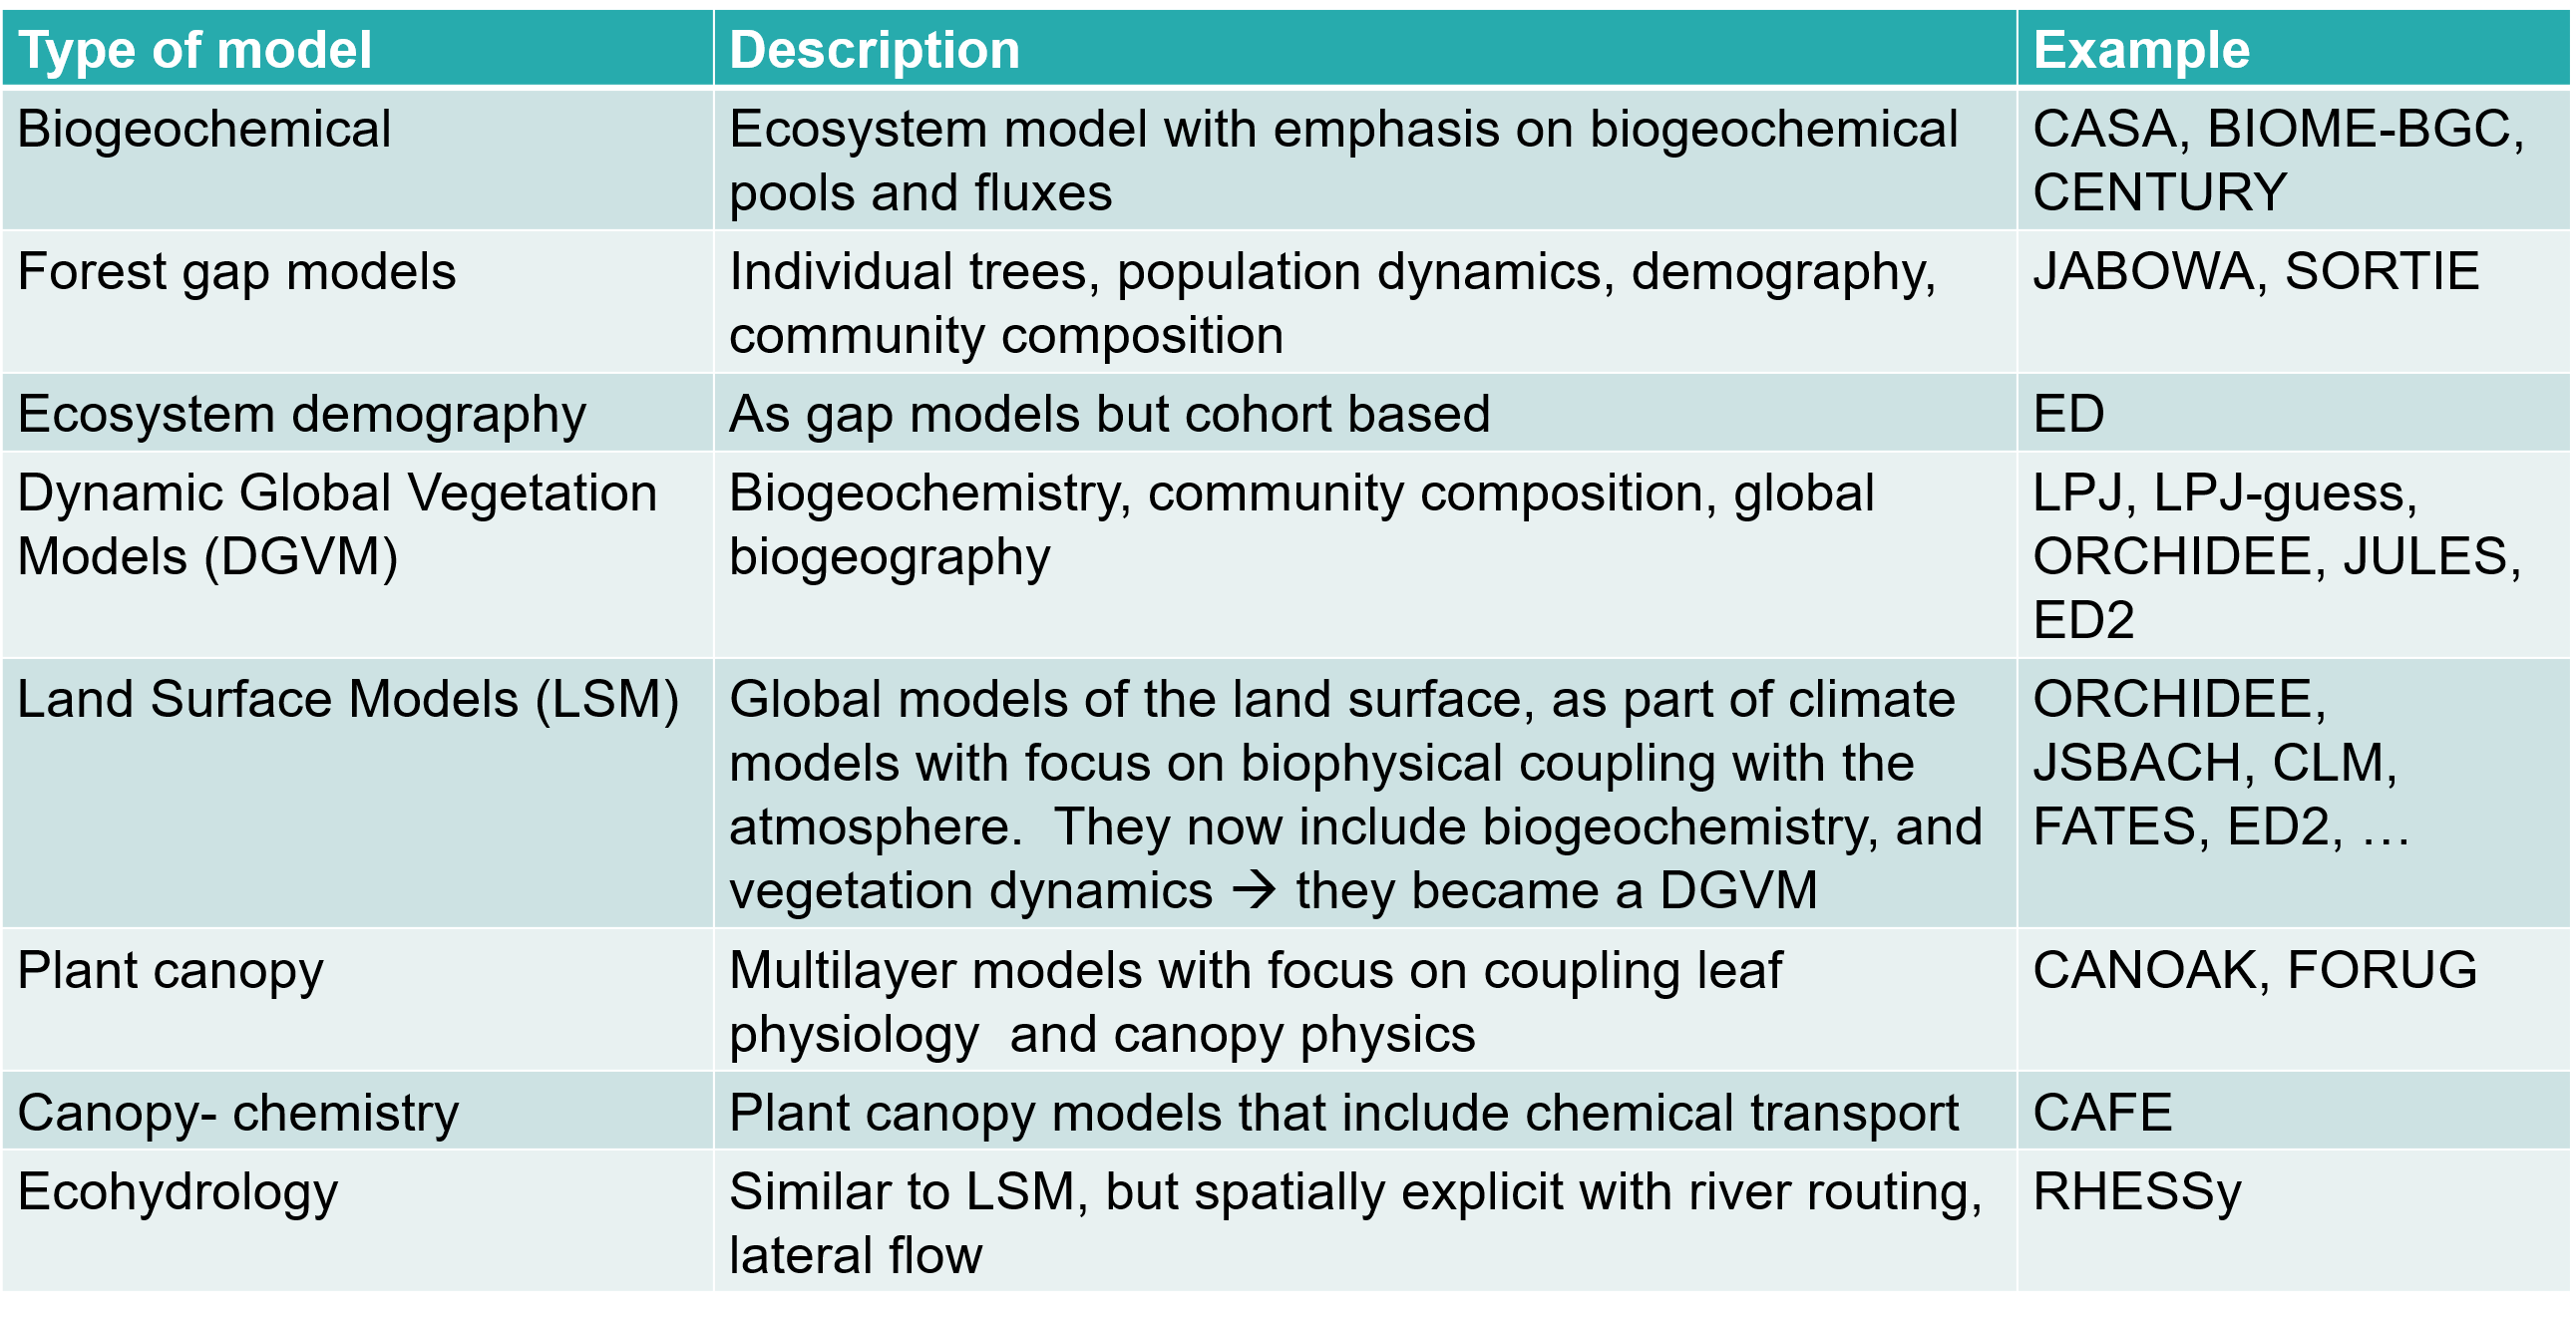
\includegraphics[width=0.8\linewidth]{figures/chap1/table_model_types} 

}

\caption{Continuum of terrestrial biosphere/ecosystem models. (Bonan 2019)}\label{fig:f5}
\end{figure}

\begin{figure}

{\centering 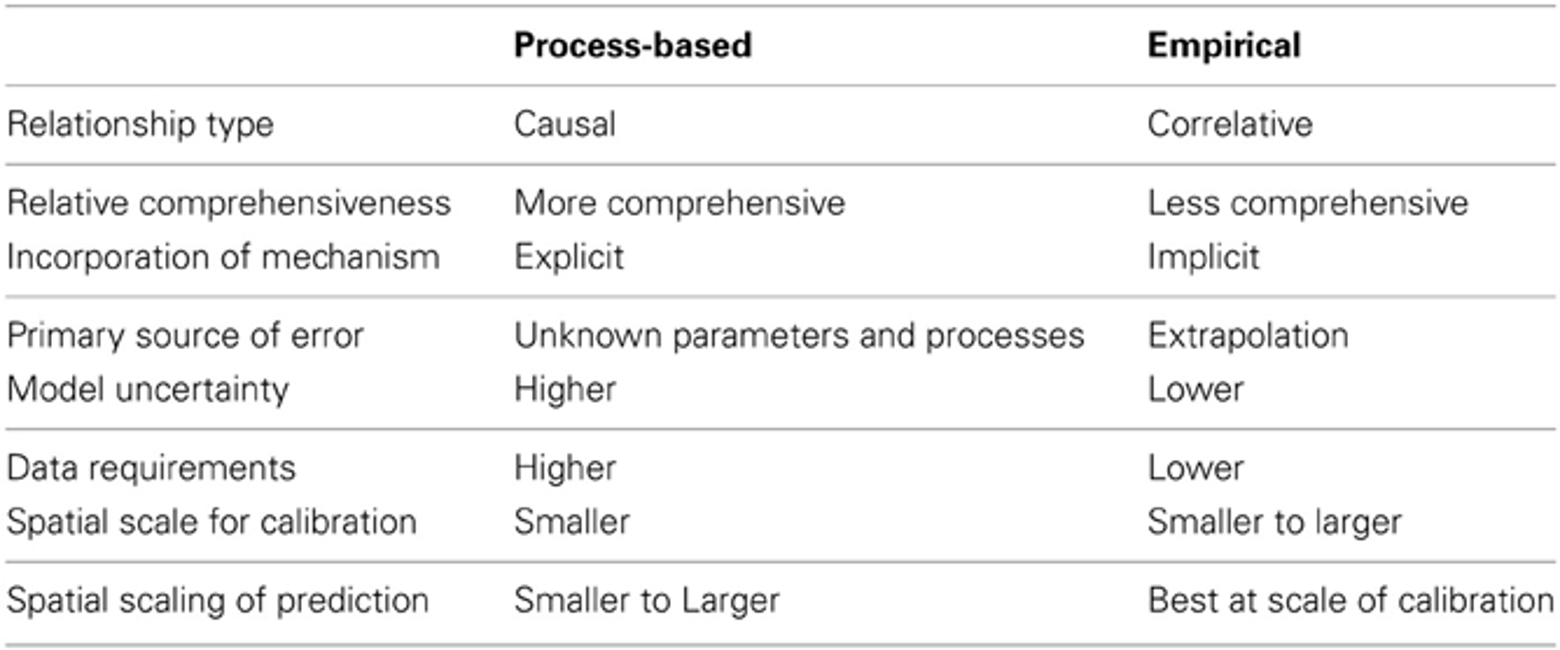
\includegraphics[width=0.8\linewidth]{figures/chap1/tables_PB_empirical} 

}

\caption{Continuum of process-based versus empirical models. (Adams et al. 2013)}\label{fig:f6}
\end{figure}

\begin{itemize}
\tightlist
\item
  continuum of terrestrial ecosystem models, from models with emphasis on biogeochemical pools and fluxes, dynamic vegetation models with focus on individual plants or size cohorts, canopy models with focus on coupling leaf physiological processes with canopy physics, and global models of the land surface for climate simulation. (Table 1.1, Bonan)
\item
  Continuum of empirical to process-based models
\item
  Types of vegetation models (depending on the purpose, questions, scales) (e.g.~timber, yield, biogeochemistry, \ldots) (ecologists, foresters, climatologist, atmospheric chemists, hydrologist all have different vegetation models\ldots)
\item
  Compare vegetation models to for example species distribution models\ldots{}
\end{itemize}

\hypertarget{the-history-of-vegetation-models}{%
\section{The history of vegetation models}\label{the-history-of-vegetation-models}}

\begin{figure}

{\centering 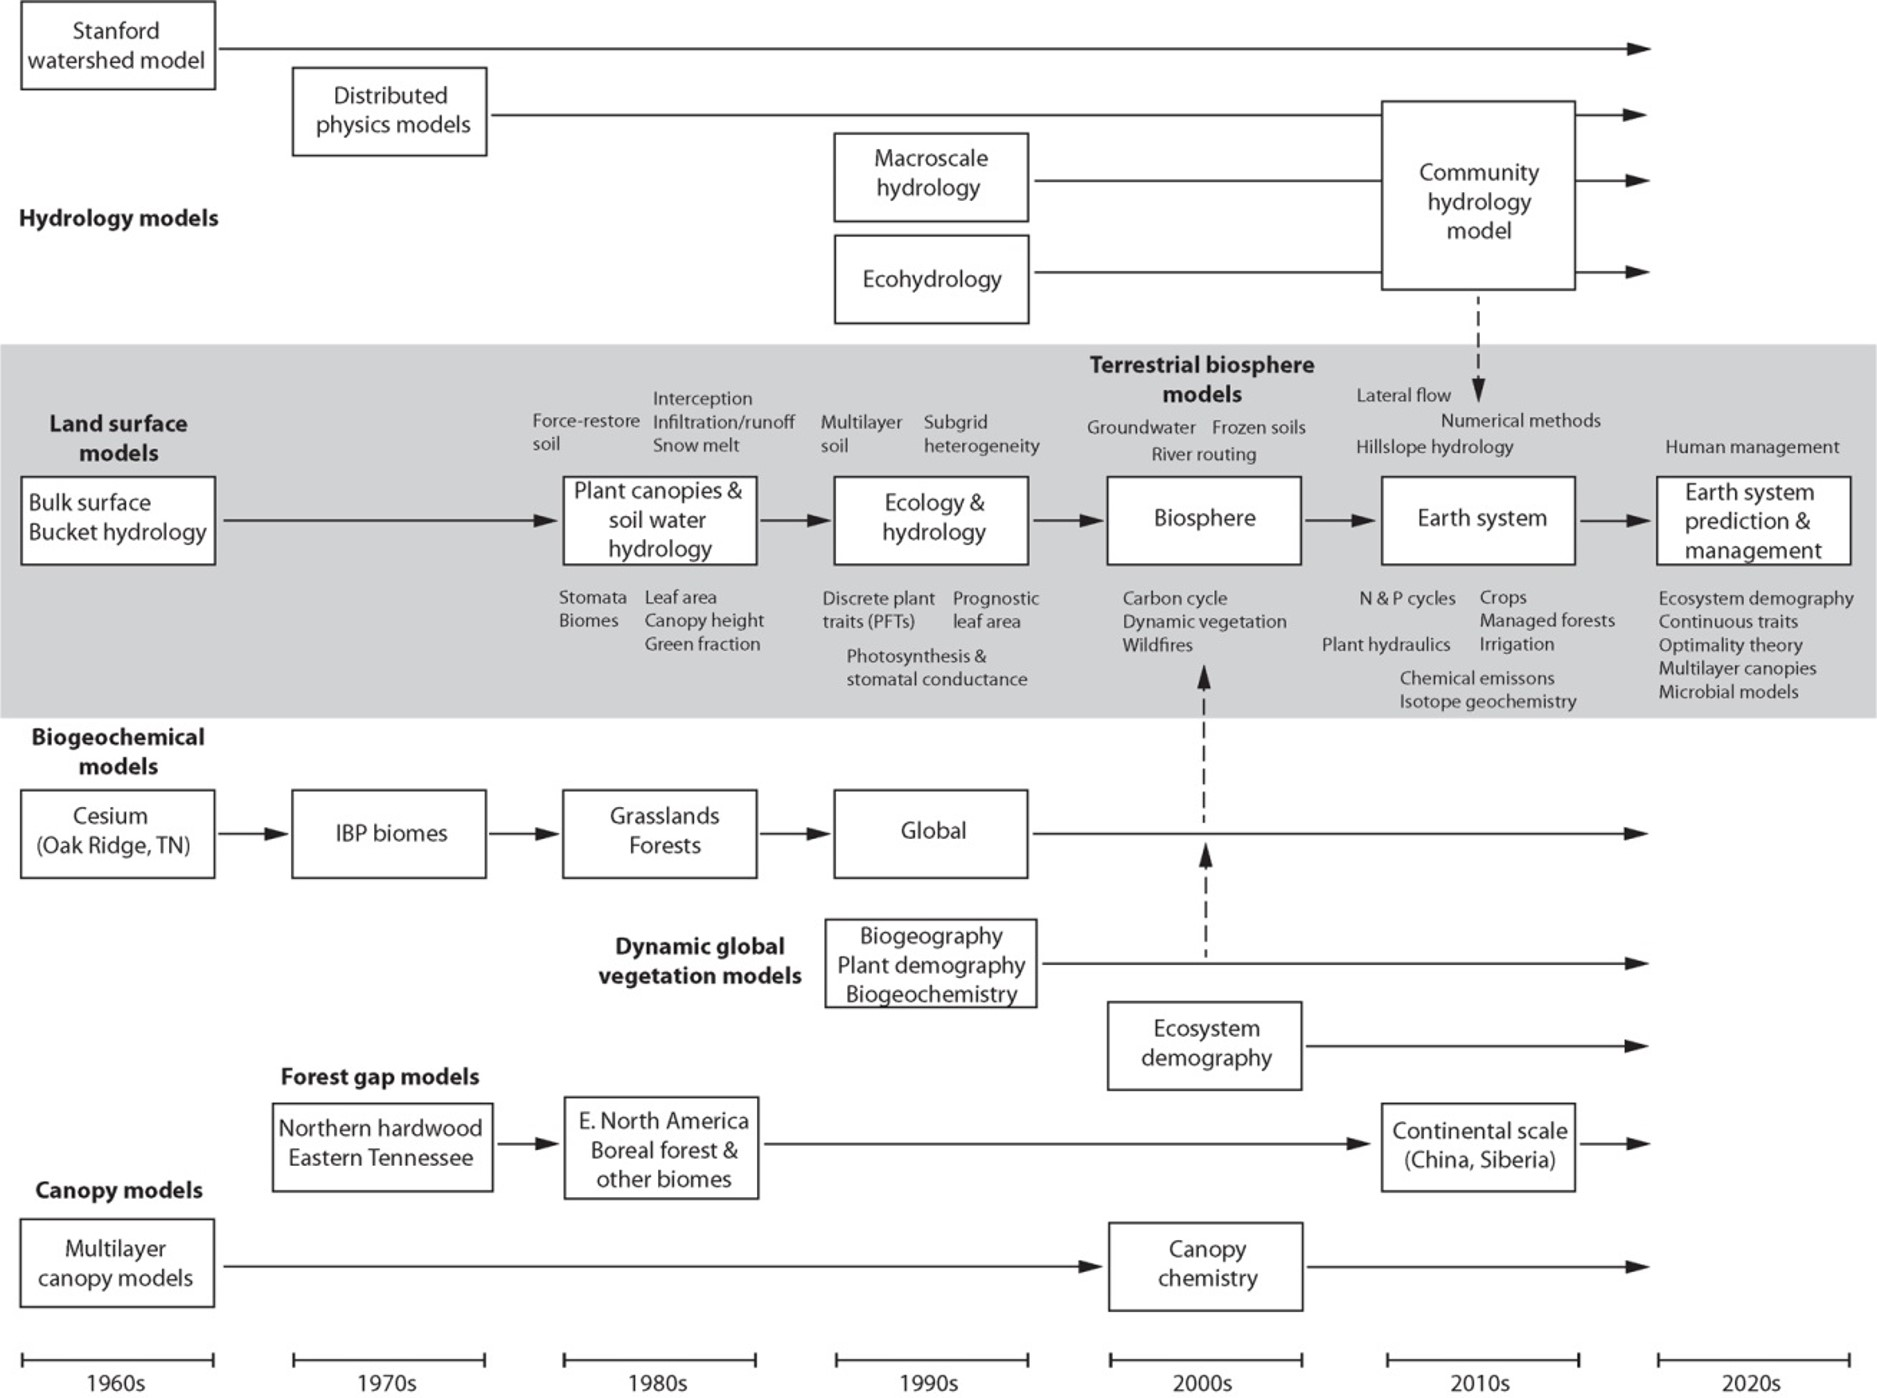
\includegraphics[width=0.8\linewidth]{figures/chap1/timeline} 

}

\caption{Timeline showing the parallel development of model types and the integration of model types into land surface models towards terrestrial biosphere models. (Bonan 2019)}\label{fig:f7}
\end{figure}

\begin{itemize}
\tightlist
\item
  Conceptualisation of ecosystem to mass and energy flows among various compartments (refer to ecology course of Steppe in the Bio-ir Bachelors. `box models in the 1960's and 1970's current global biogeochemical models are still box-type of models (Fig 1.4)
\item
  In parallel individual based models of forest dynamics were developed, based on population dynamics, life cycle of species. They are also called ``gap models'' that simulate the demography in an area of 0.1 ha (size of a gap in the canopy) (Fig 1.5). Ecosystem properties such as carbon stocks are emerging from the demography simulation.
\item
  More recently cohort based models
\item
  DGVMs: These models also simulate changes in community composition, biomass, productivity, and nutrient cycling. Because the models are applied globally, they do not recognize individual species. Rather, they employ plant functional types, Table 1.2
\item
  Fig 1.2 Bonan
\end{itemize}

\hypertarget{components-of-a-model}{%
\section{Components of a model}\label{components-of-a-model}}

\begin{figure}

{\centering 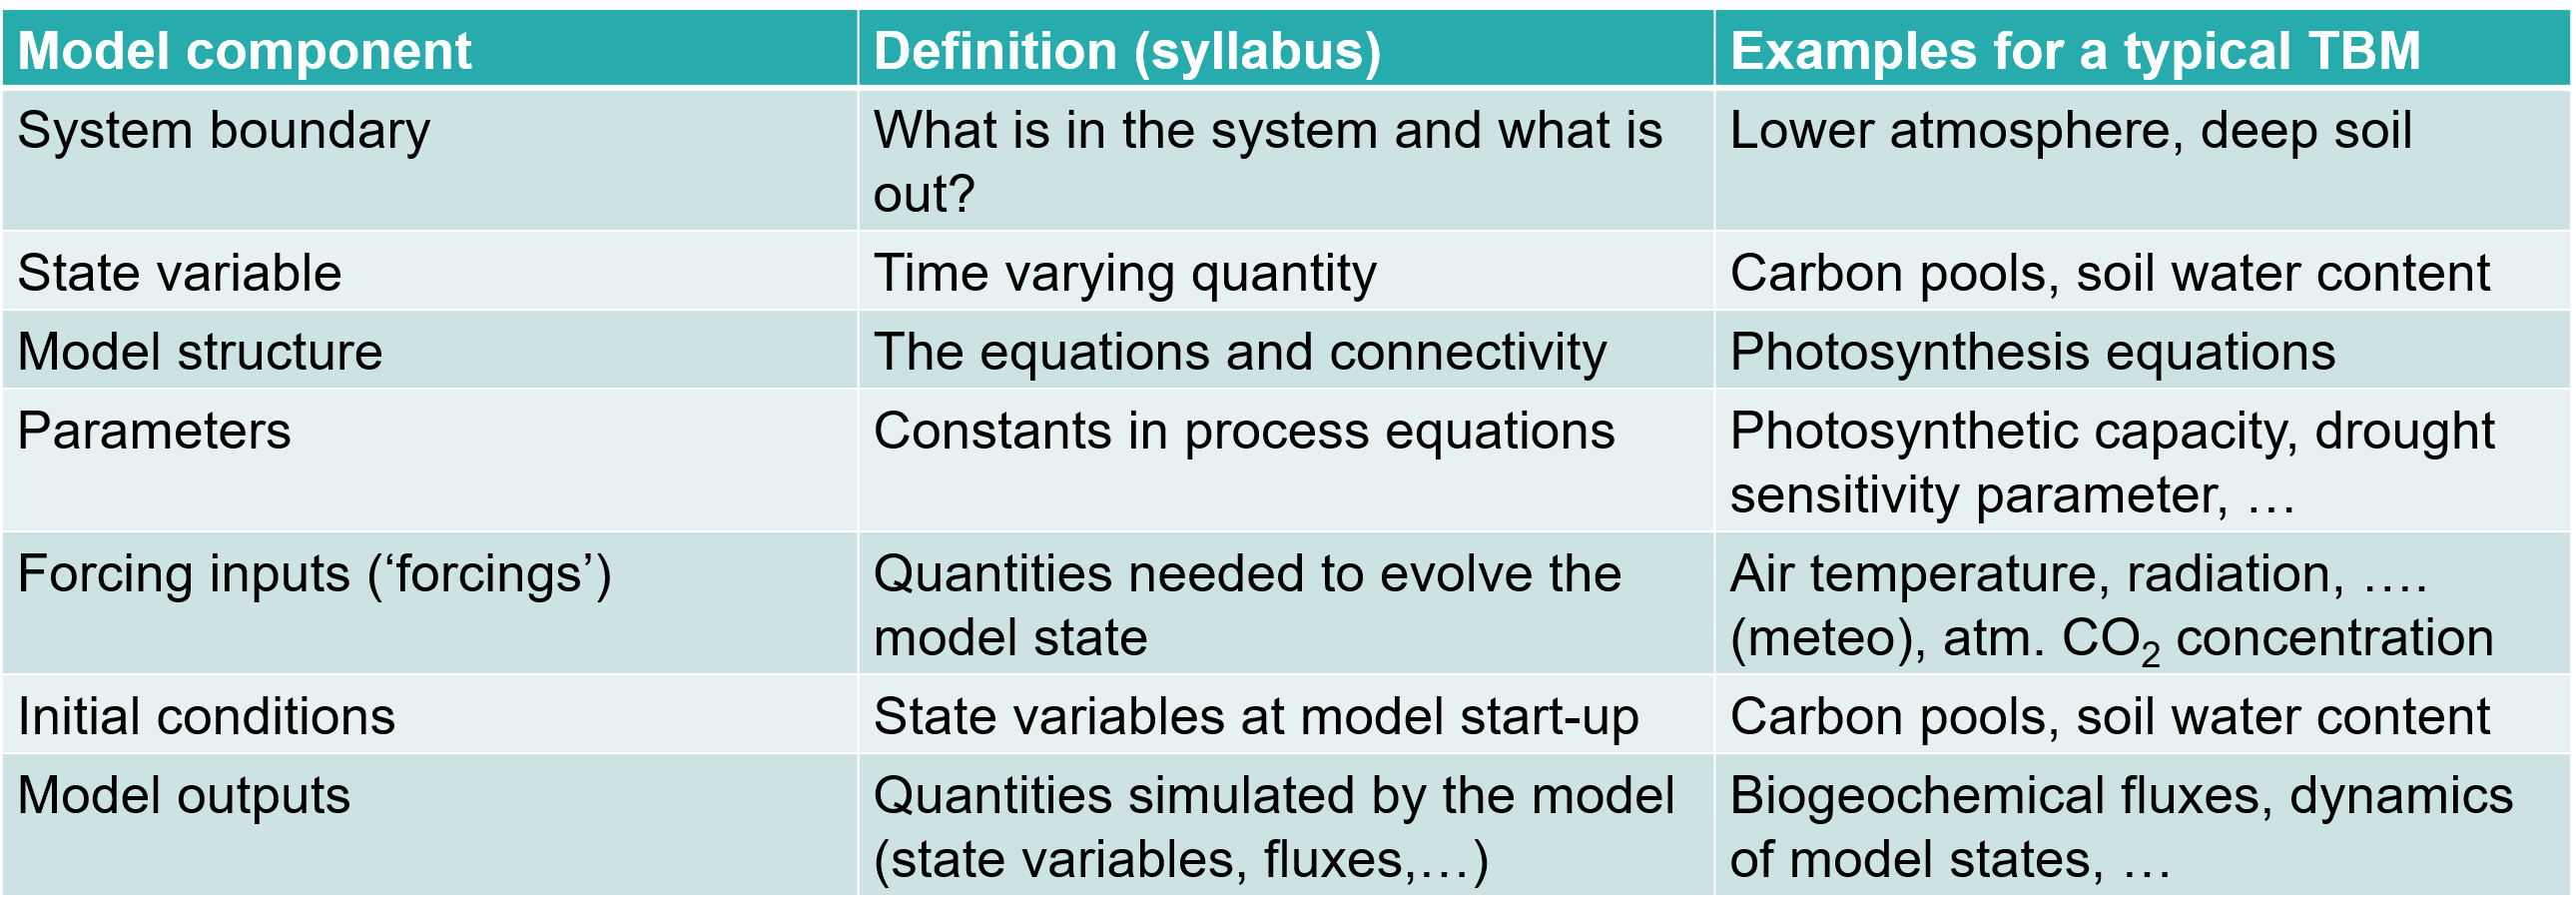
\includegraphics[width=0.8\linewidth]{figures/chap1/table_components} 

}

\caption{Definition of key model components and examples for a typical TBM}\label{fig:f8}
\end{figure}

\begin{figure}

{\centering 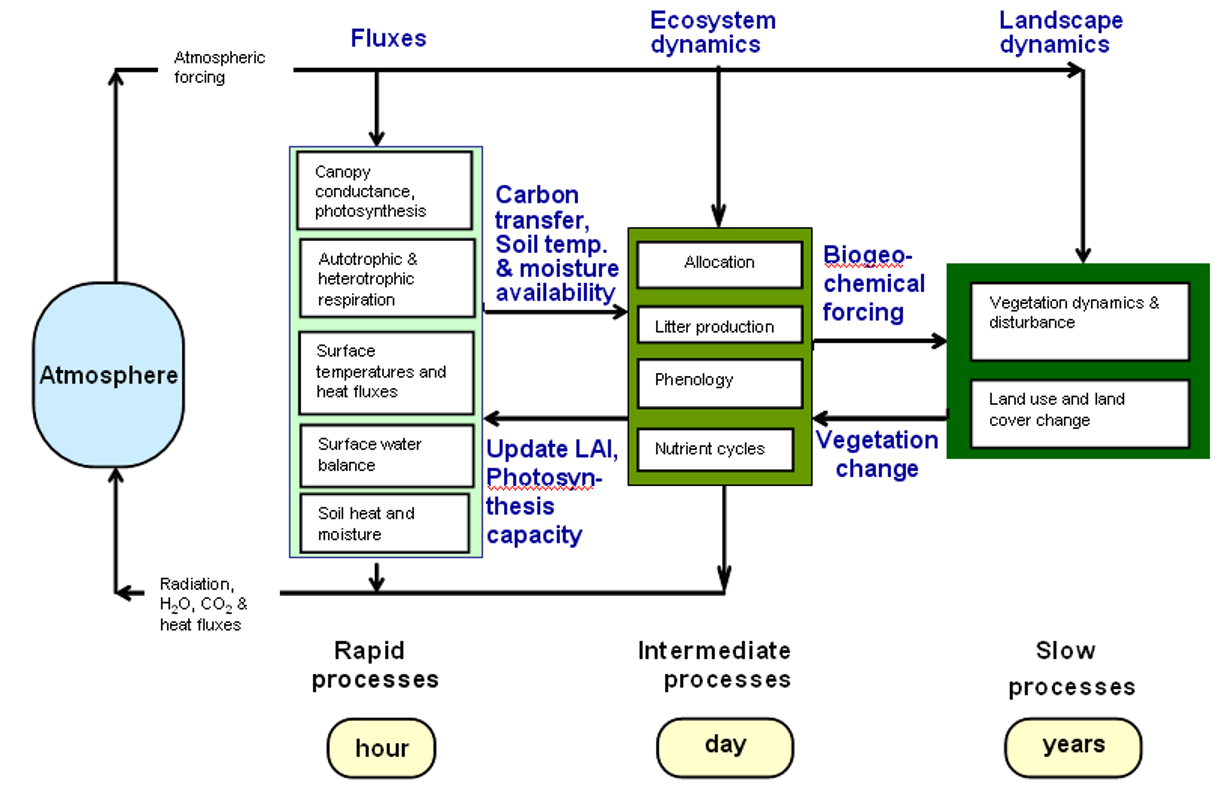
\includegraphics[width=0.8\linewidth]{figures/chap1/time_steps} 

}

\caption{Structure of a vegattion model indicating the different time steps at which each process is simulated (Williams et al. 2009)}\label{fig:f9}
\end{figure}

\begin{figure}

{\centering 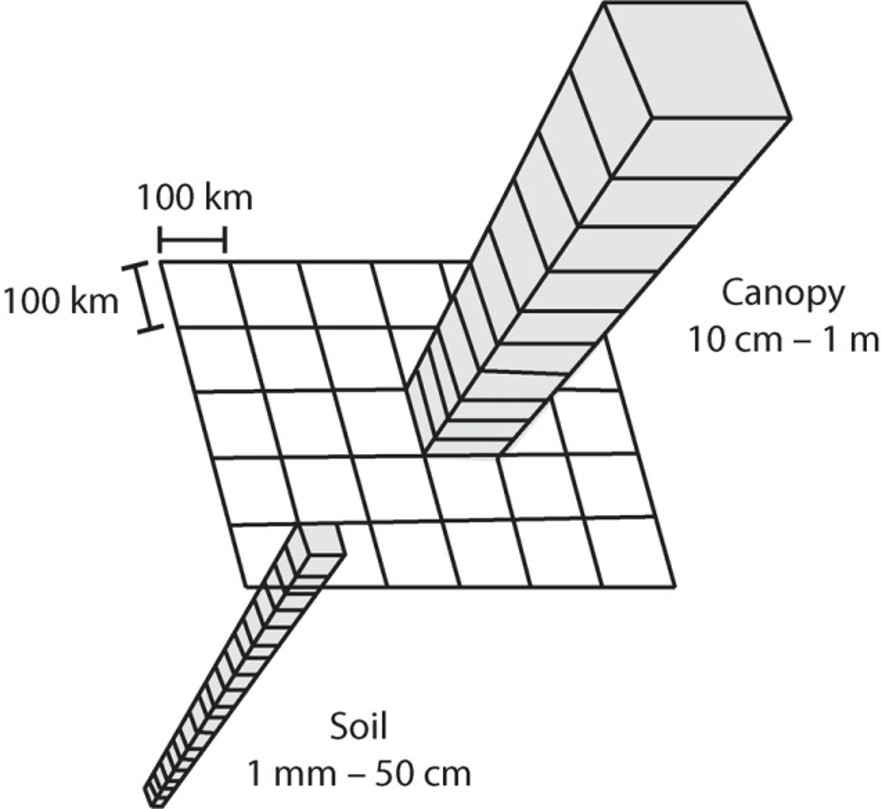
\includegraphics[width=0.8\linewidth]{figures/chap1/grid_vert_hor} 

}

\caption{Three dimensional grid of a TBM structured in terms of longitude x latitude x level. The number of soil and canopy layers and the geographical resolution is model dependent, (Bonan 2019)}\label{fig:f10}
\end{figure}

\begin{figure}

{\centering 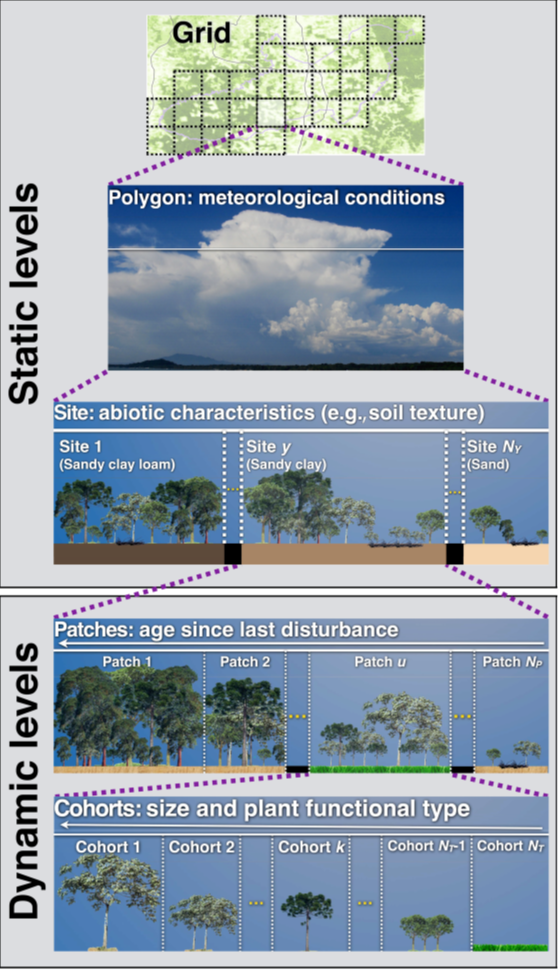
\includegraphics[width=0.8\linewidth]{figures/chap1/grid_ED2} 

}

\caption{Example: the spatial multi-level grid structure of of the ED2 vegetation model (Longo et al. 2019)}\label{fig:f11}
\end{figure}

\begin{itemize}
\tightlist
\item
  Table 1.3 and Table 1.4
\item
  Model structure (constraints: resolving of fluxes on short time scales, conservation of mass and energy,
\item
  Parameters
\item
  i/o variables, state variable
\item
  time steps (fluxes must be resolved on a short time interval, diurnal cycles)
\item
  spatial structure (Fig 1.11)
\item
  Prognostic equations use time derivatives to describe the change in a state variable and are integrated forward in time from some initial condition. Prognostic variables must be numerically stepped forward from time n to n + 1 over the time interval deltat.
\item
  Conservation equations
\item
  Diagnostic equations (e.g.~ideal gas law) linking variables time-independent
\item
  Initial conditions
\item
  Model code, There is an enormous leap between seeing a mathematical equation in a research paper and actually using that equation in a model (Bonan Book).
\item
  Model uncertainty and complexity (fig 1.12) (+ fig from Dietze book)
\end{itemize}

\hypertarget{modelling-workflow-and-structure-of-the-course}{%
\section{Modelling workflow and structure of the course}\label{modelling-workflow-and-structure-of-the-course}}

\begin{figure}

{\centering 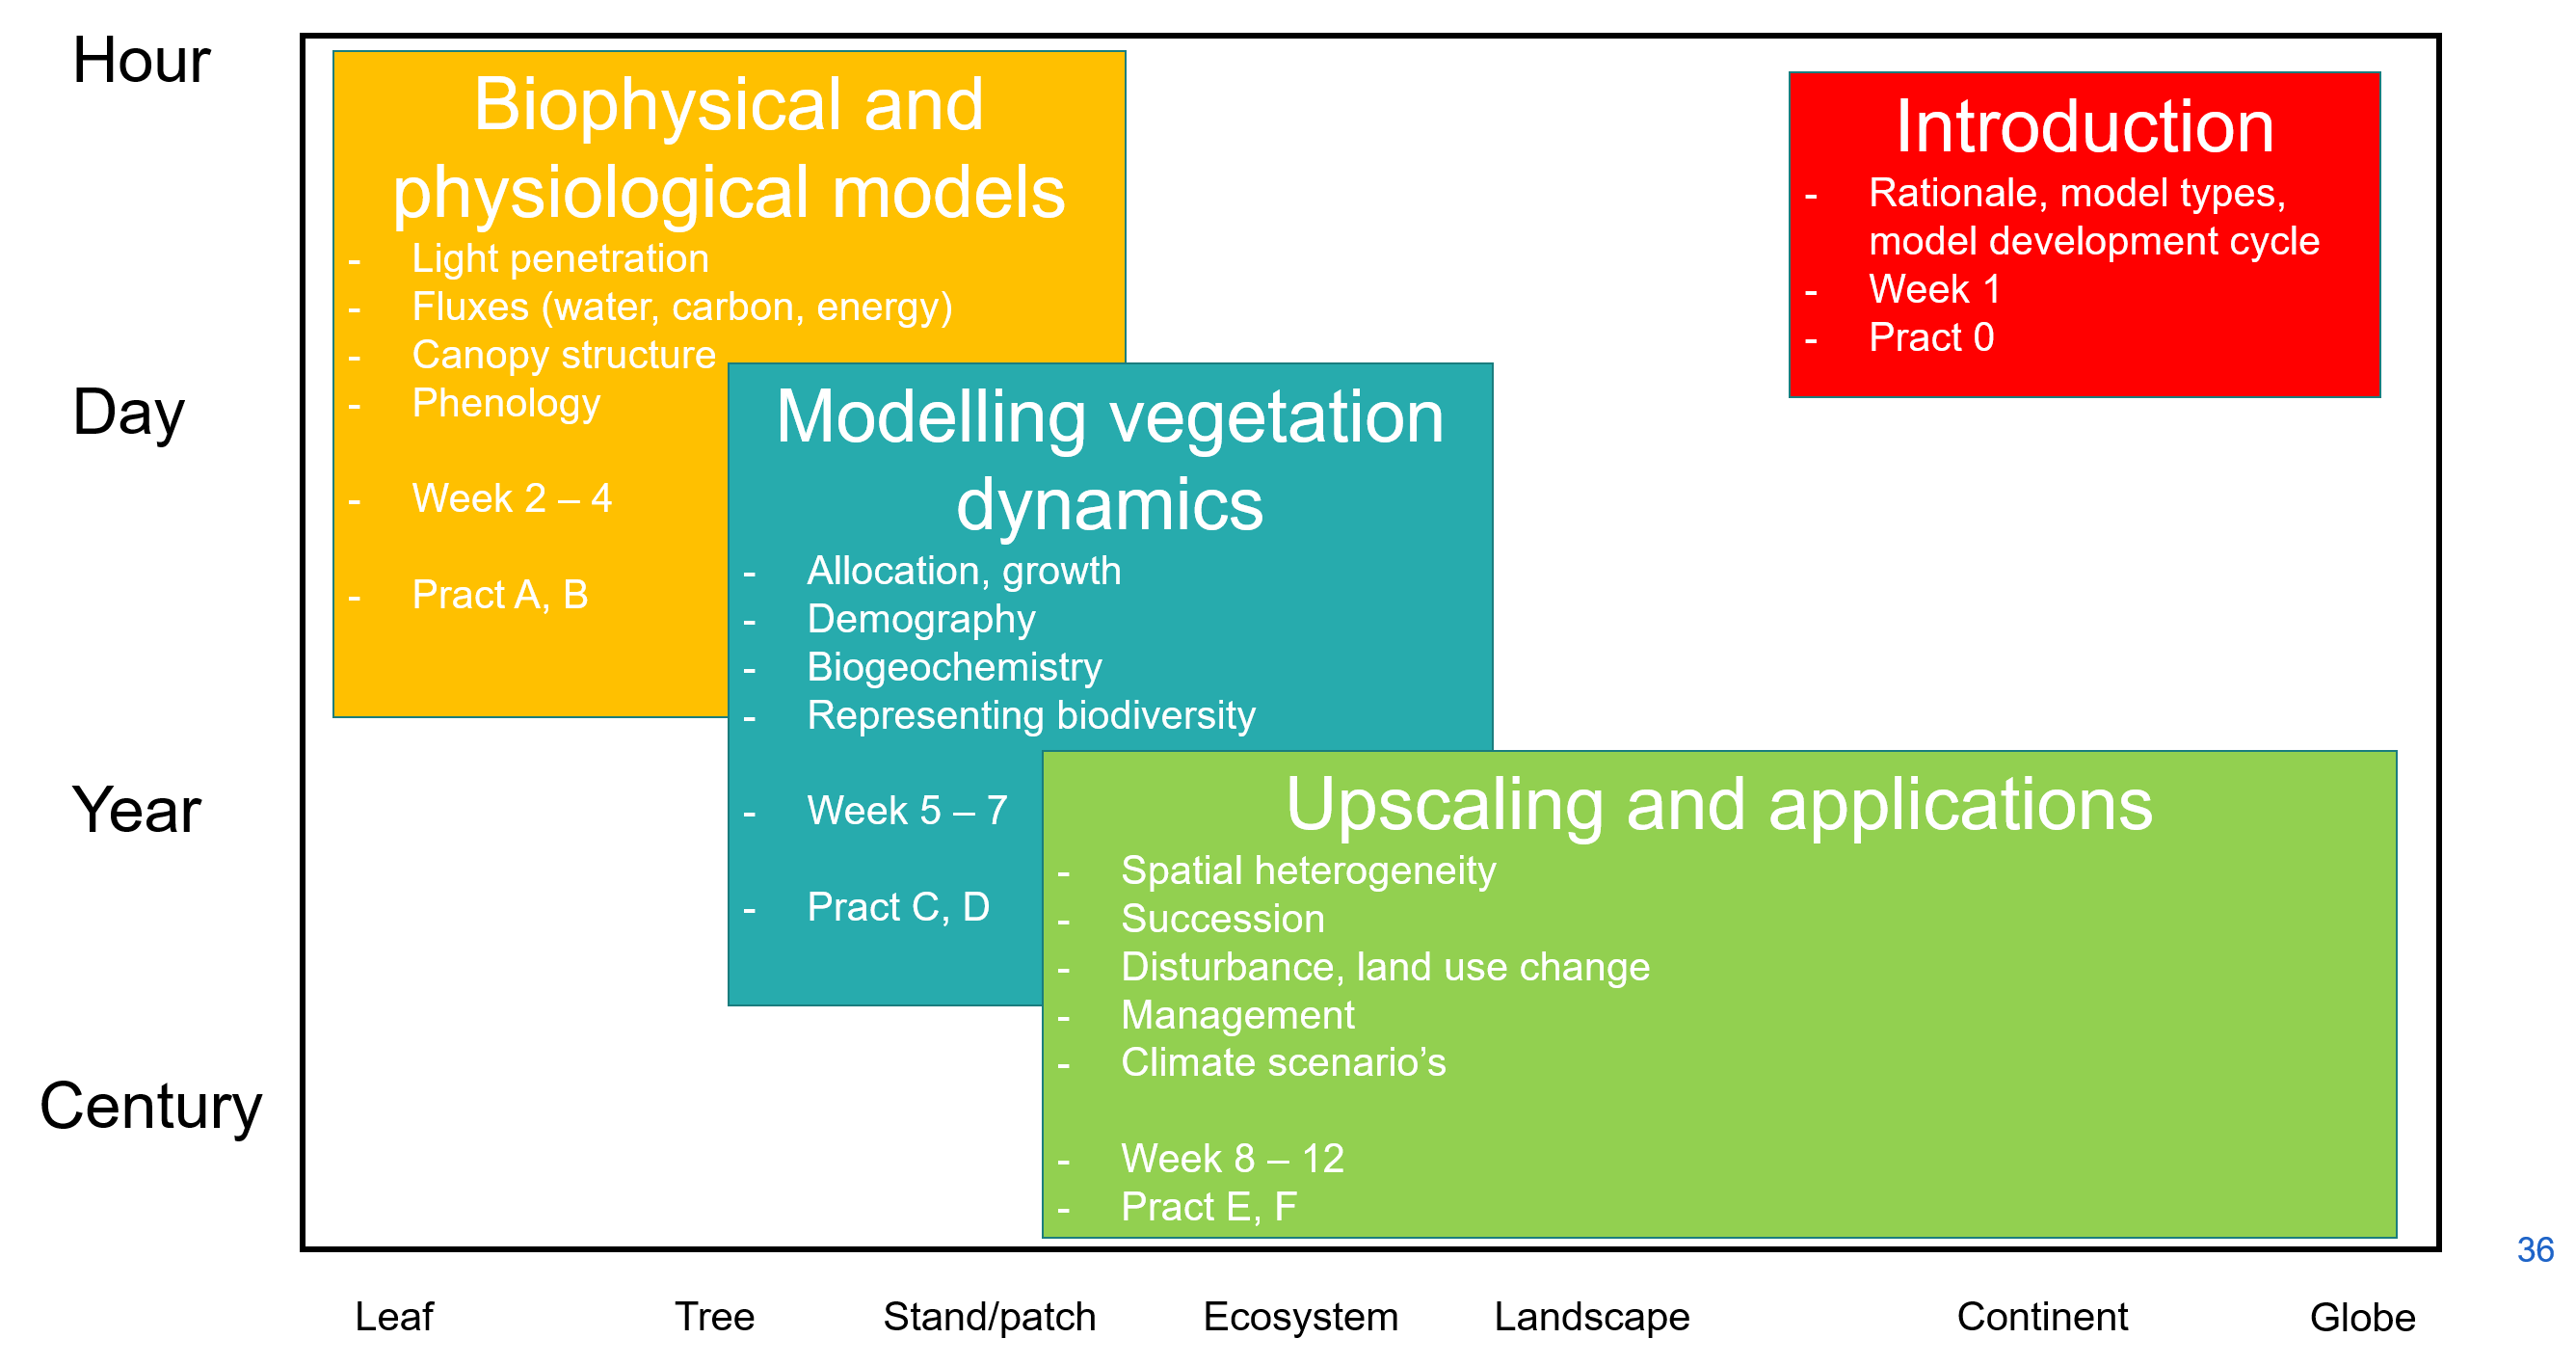
\includegraphics[width=0.8\linewidth]{figures/chap1/course_overview} 

}

\caption{Progression through spatial and temporal scales throughout this course}\label{fig:f12}
\end{figure}

\begin{figure}

{\centering 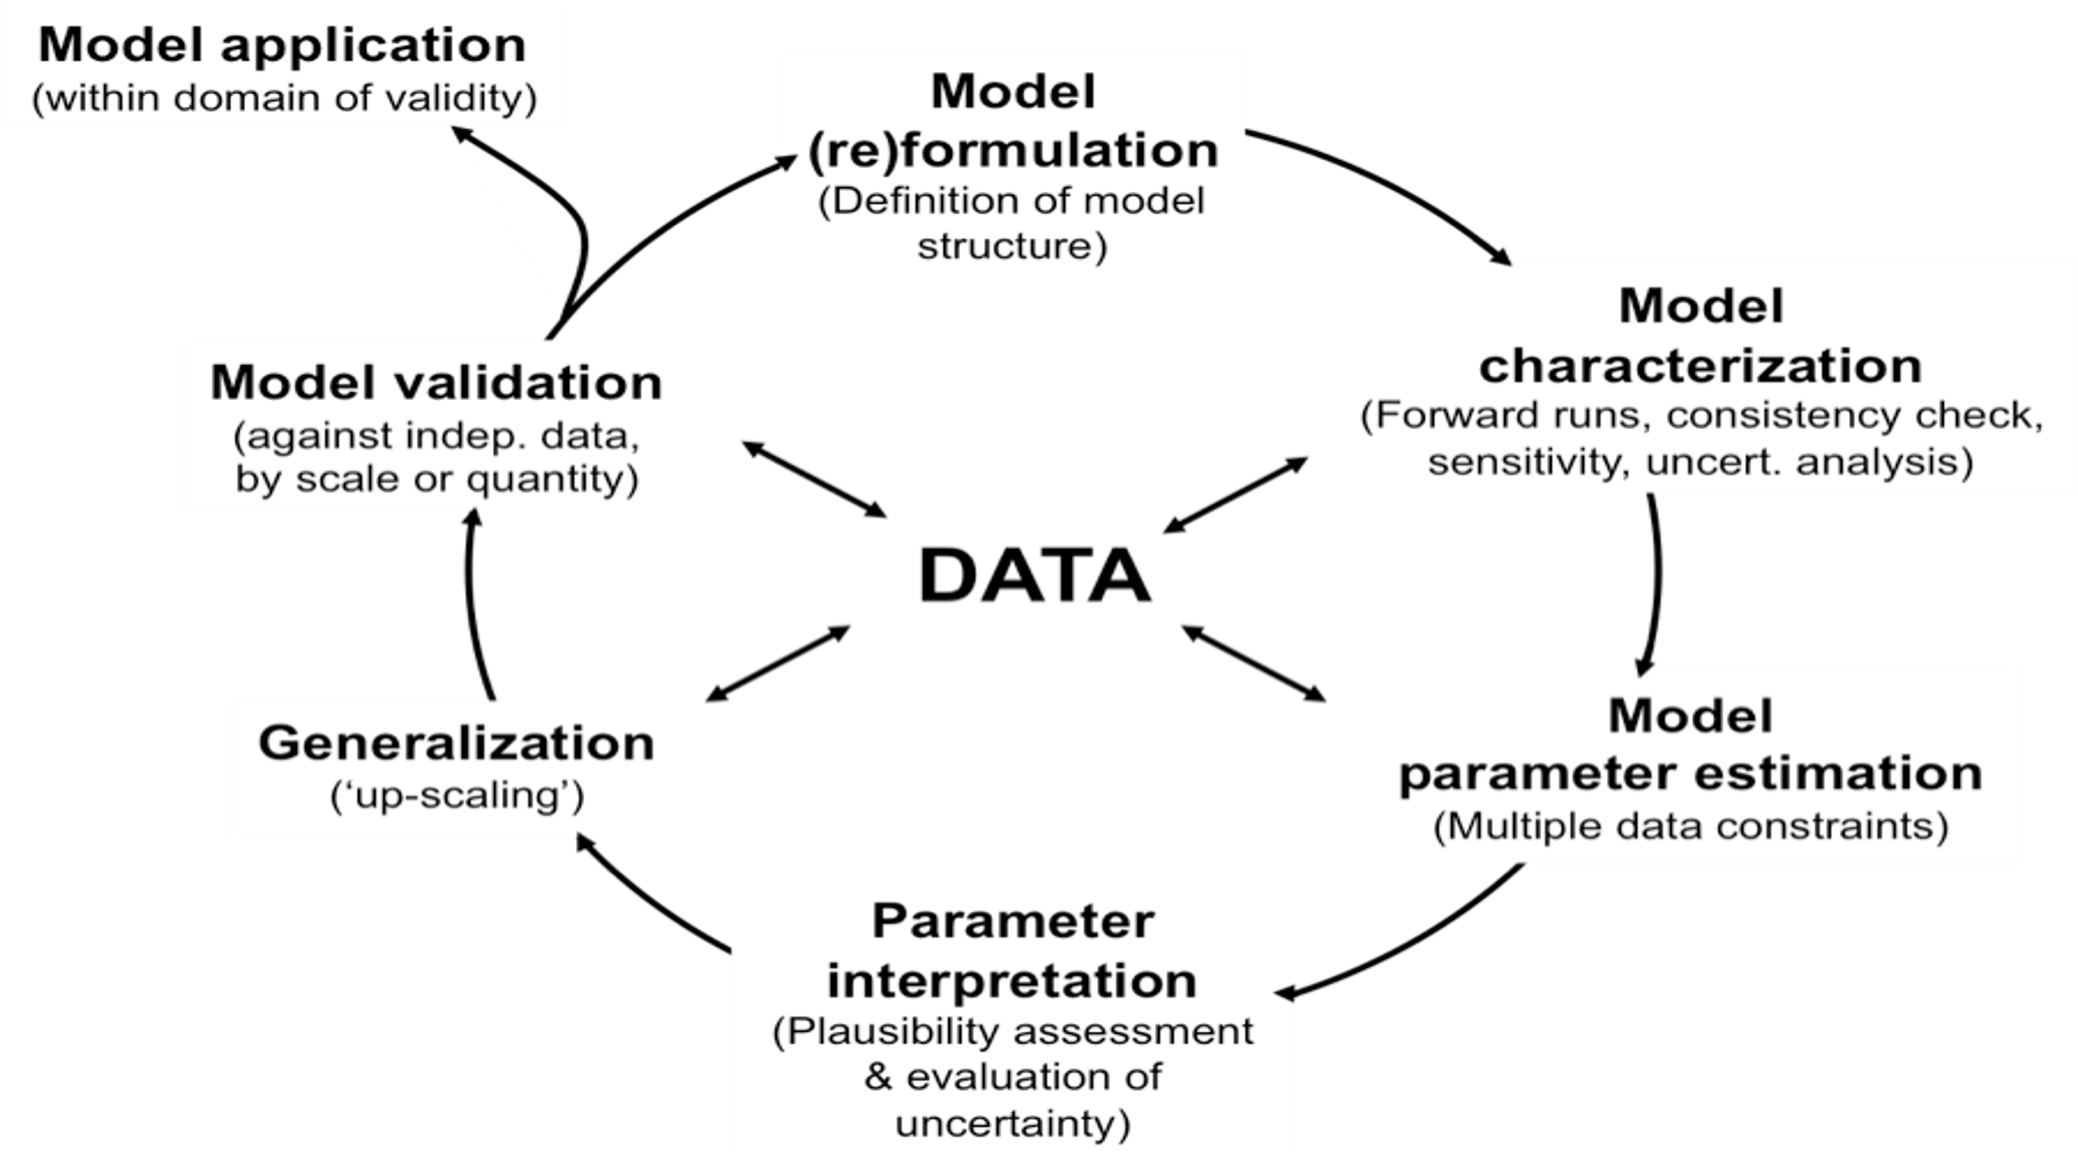
\includegraphics[width=0.8\linewidth]{figures/chap1/williams_fusion} 

}

\caption{Model data fusion in every step of the model development cycle (Williams et al. 2009)}\label{fig:f13}
\end{figure}

\begin{figure}

{\centering 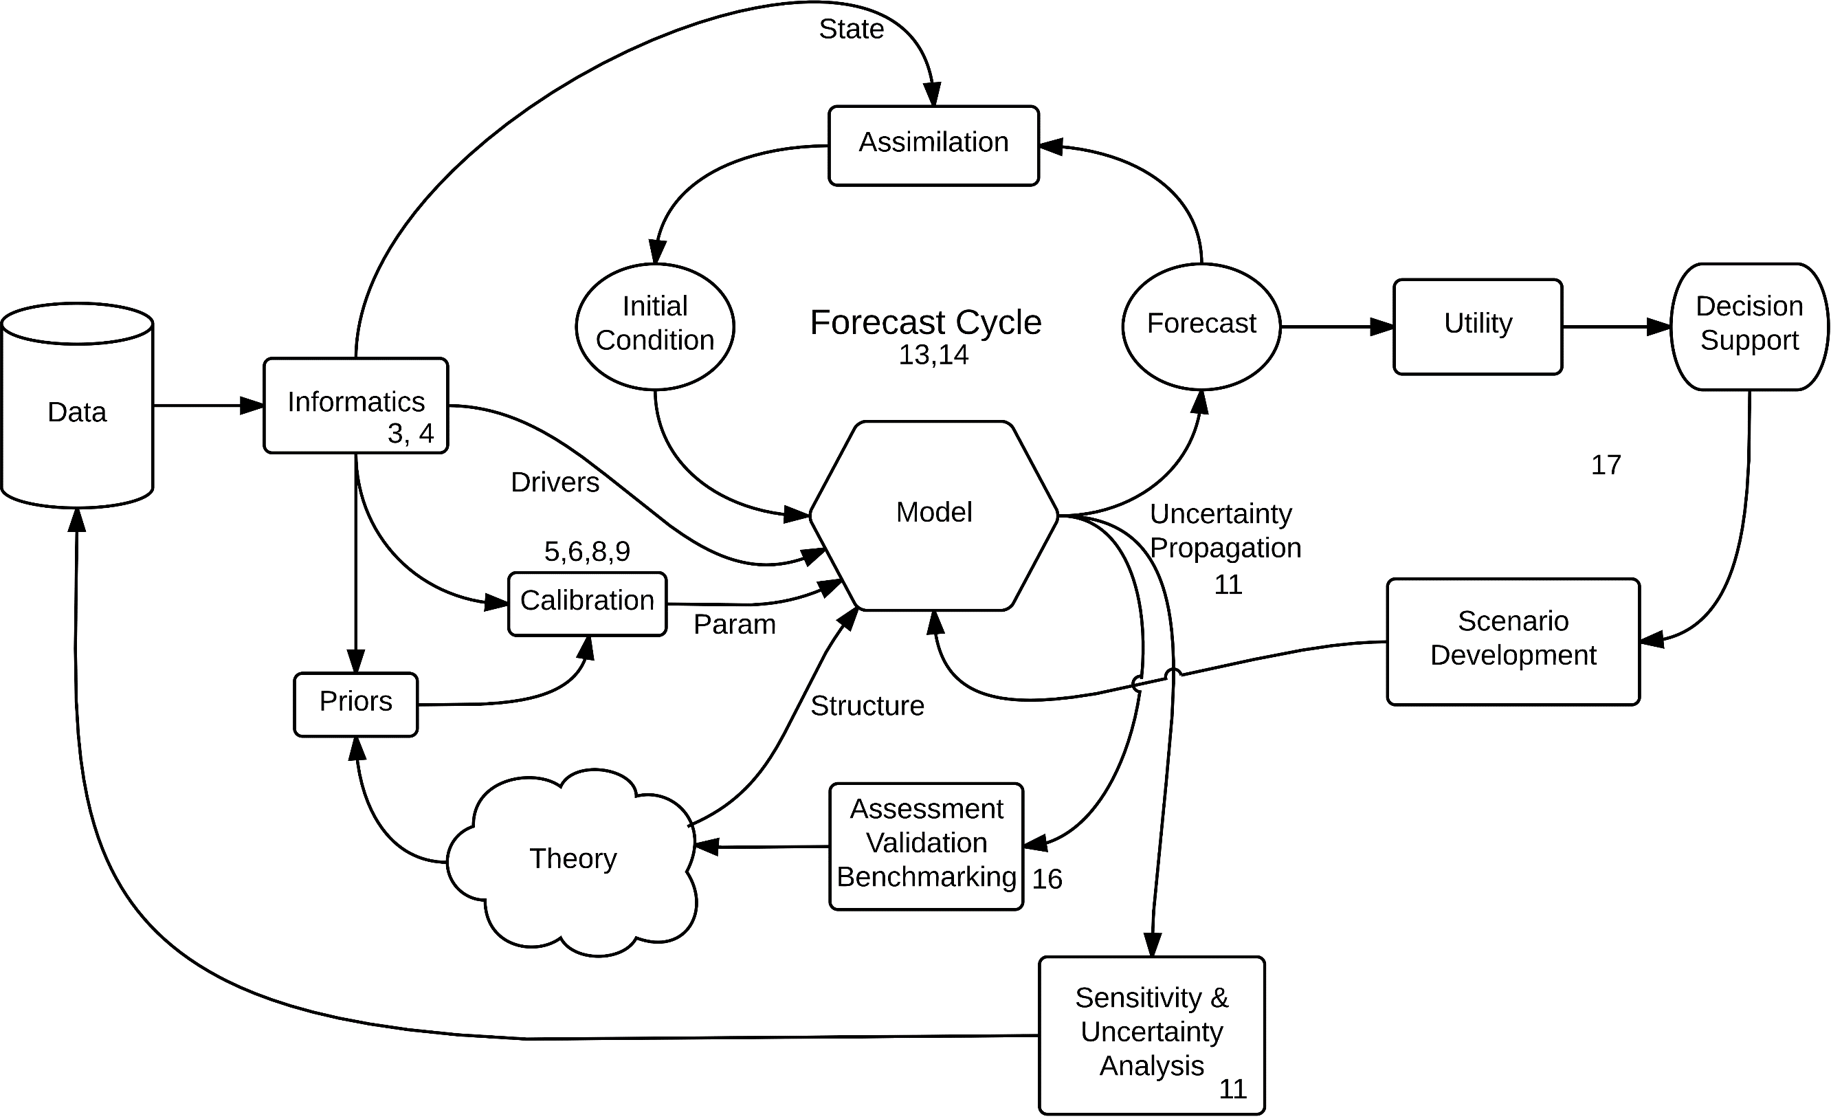
\includegraphics[width=0.8\linewidth]{figures/chap1/dietze_workflow} 

}

\caption{Methodological workflow of model data fusion (Dietze: Ecological Forecasting)}\label{fig:f14}
\end{figure}

\begin{itemize}
\tightlist
\item
  a science that spans boundary layer meteorology, micrometeorology, atmospheric chemistry, plant physiology, ecosystem ecology, biogeochemistry, soil science, hydrology, and geochemistry \ldots{} we will not discuss all the basics in this course, but we expect you to know from other courses (Ecology, plant physiology, forestry, hydrology, soil science \ldots), but we will of course go into the processes, but focus on there mathematical formulation and translation into a workin model (code)
\item
  progression through the course (space-time figure, with chapters)
\item
  Model development cycle (structure for the methodological focus of each application/practical) (Dietze figure)
\end{itemize}

\textbf{to test: Idea of a conceptual figure that we will build block by block as we go deeper in the course. It represents the concept that vegetation modelling is to have an integrated representation of the plant functioning and all the underlying processes at different scales. }

\hypertarget{part-biophysical-and-physiological-models}{%
\part{Biophysical and physiological models}\label{part-biophysical-and-physiological-models}}

\hypertarget{modelling-plant-basic-processes}{%
\chapter{Modelling plant basic processes}\label{modelling-plant-basic-processes}}

\chaptermark{photsynthesis}

\textbf{For all processes, we provide an overview of existing models and approaches and we will detail only one of them for the practical course. This also apply for the other chapters, the idea of the course is to be more conceptual about how we model vegetation and the different applications and assumptions.}

\hypertarget{photosynthesis}{%
\section{Photosynthesis}\label{photosynthesis}}

\hypertarget{c3-photosynthesis}{%
\subsection{C3 photosynthesis}\label{c3-photosynthesis}}

\begin{itemize}
\tightlist
\item
  UCL 4.6.1
\item
  Bonan, Chapter 11.1
  The FvCB model
  Most equations between 11.1 and 11.31
  Figure 11.2 a and b
  Table 11.1 for parameters values + a few simulations to illustrate
  Table 11.4
\end{itemize}

\hypertarget{parameter-and-temperature-dependencies}{%
\subsection{Parameter and temperature dependencies}\label{parameter-and-temperature-dependencies}}

\begin{itemize}
\tightlist
\item
  Bonan, Chapter 11.2
  Equations 11.34-11.37
  Table 11.2
  Figure 11.3 for illustration
\end{itemize}

Summary with Table 11.5 and Figure 11.4

\hypertarget{c4-photosynthesis}{%
\subsection{C4 photosynthesis}\label{c4-photosynthesis}}

\begin{itemize}
\tightlist
\item
  Bonan, Chapter 11.7
  PEP carboxylase
  Equations 11.69-11.74
  Find an illustration
\end{itemize}

\hypertarget{respiration-models}{%
\section{Respiration models}\label{respiration-models}}

-Q10 etc\ldots{}
-leaf respiration
-woody respiration
-Soil respiration → see chapter 7

\hypertarget{transpiration-and-stomatal-models}{%
\section{Transpiration and stomatal models}\label{transpiration-and-stomatal-models}}

\hypertarget{penman-monteith-equation}{%
\subsection{Penman-Monteith equation}\label{penman-monteith-equation}}

\begin{itemize}
\tightlist
\item
  Bonan, Chapter 7.6
\end{itemize}

\hypertarget{stomatal-conductance}{%
\subsection{Stomatal conductance}\label{stomatal-conductance}}

\begin{itemize}
\tightlist
\item
  stomatal models (Jarvis, Ball-Berry, Leuning, \ldots)
\item
  Bonan, Chapter 12.2-3
\end{itemize}

Figure 12.1-12.2 and Equations 12.1-12.5
Summary Table 12.1

\hypertarget{empirical-multiplicative-models}{%
\subsubsection{Empirical multiplicative models}\label{empirical-multiplicative-models}}

\begin{itemize}
\tightlist
\item
  Bonan, Chapter 12.2
\end{itemize}

\hypertarget{semiempirical-photosynthesis-based-models}{%
\subsubsection{Semiempirical photosynthesis-based models}\label{semiempirical-photosynthesis-based-models}}

\begin{itemize}
\tightlist
\item
  Bonan, Chapter 12.3
\end{itemize}

\hypertarget{wue-model}{%
\subsubsection{WUE model}\label{wue-model}}

\begin{itemize}
\tightlist
\item
  Bonan, Chapter 12.4 + add optimality approach from Prentice et al.
\end{itemize}

\hypertarget{hydraulic-models}{%
\subsubsection{Hydraulic models}\label{hydraulic-models}}

Figure 13.1
The soil-plant-atmosphere model
Leaf water potential
Plant water uptake
Resistance analogy
Multinode models

\hypertarget{stomatal-response-to-environmental-factors}{%
\subsection{Stomatal response to environmental factors}\label{stomatal-response-to-environmental-factors}}

\begin{itemize}
\tightlist
\item
  Bonan, Chapter 12.5
\item
  Bonan, Chapter 12.7
\end{itemize}

\hypertarget{upscaling-from-leaf-to-canopy}{%
\section{Upscaling from leaf to canopy}\label{upscaling-from-leaf-to-canopy}}

\begin{itemize}
\tightlist
\item
  Quickly introduce the problem of scaling in ecology (review paper of Jerome Chave) and refer to chapter 10 on upscalling
\item
  Canopy integration: LAI layers, etc\ldots{} Nice transition to chap 3 with the interception of light by the canopy
\end{itemize}

\hypertarget{modelling-light-penetration-vegetation-canopy-representation-and-energy-balance}{%
\chapter{Modelling light penetration, vegetation canopy representation, and energy balance}\label{modelling-light-penetration-vegetation-canopy-representation-and-energy-balance}}

\chaptermark{Light}

\begin{itemize}
\tightlist
\item
  Mainly Chapter 14 from Bonan
\end{itemize}

\hypertarget{introduction}{%
\section{Introduction}\label{introduction}}

\begin{itemize}
\tightlist
\item
  Bonan, Chapter 14.1
  Figure 14.1
  Figure 14.2
\end{itemize}

\hypertarget{radiative-transfer-modelling}{%
\section{Radiative transfer modelling}\label{radiative-transfer-modelling}}

\hypertarget{leaf-optical-properties}{%
\subsection{Leaf optical properties}\label{leaf-optical-properties}}

\begin{itemize}
\tightlist
\item
  Bonan, Chapter 14.2
  Example of leaf spectrum
  Prospect model
  Example of parameters 14.2 + simulations/analysis of sensitivity
\end{itemize}

\hypertarget{light-transmission-without-scattering}{%
\subsection{Light transmission without scattering}\label{light-transmission-without-scattering}}

\begin{itemize}
\tightlist
\item
  The Beer-Bouguer-Lambert law
\item
  Bonan, Chapter 14.3
  Most of quations 14.2-14.17 for model description
  Figure 14.4 and Figure 14.5
\end{itemize}

\hypertarget{direct-beam-extinction-coefficient}{%
\subsection{Direct beam extinction coefficient}\label{direct-beam-extinction-coefficient}}

\begin{itemize}
\tightlist
\item
  Could be skipped
\item
  Bonan, Chapter 14.4
\end{itemize}

\hypertarget{diffuse-transmittance}{%
\subsection{Diffuse transmittance}\label{diffuse-transmittance}}

\begin{itemize}
\tightlist
\item
  Bonan, Chapter 14.5
  Figure 14.12
\end{itemize}

\hypertarget{the-norman-model}{%
\subsection{The Norman Model}\label{the-norman-model}}

\begin{itemize}
\tightlist
\item
  Bonan, Chapter 14.6
\item
  Numerical
  Figure 14.15
\end{itemize}

\hypertarget{the-goudriaan-and-van-laar-model}{%
\subsection{The Goudriaan and van Laar Model}\label{the-goudriaan-and-van-laar-model}}

\begin{itemize}
\tightlist
\item
  Bonan, Chapter 14.7
\item
  Analytical
  Figure 14.16 + 14.15 and 14.17 for comparison with the Norman model
\end{itemize}

\hypertarget{the-two-stream-approximation}{%
\subsection{The Two-Stream approximation}\label{the-two-stream-approximation}}

\begin{itemize}
\tightlist
\item
  Bonan, Chapter 14.8
  Figure 14.19 + simulations
\end{itemize}

\hypertarget{surface-albedo}{%
\subsection{Surface Albedo}\label{surface-albedo}}

\begin{itemize}
\tightlist
\item
  Bonan, Chapter 14.9
  Figure 14.20 and Figure 14.21
\end{itemize}

\hypertarget{longwave-radiation}{%
\subsection{Longwave radiation}\label{longwave-radiation}}

\begin{itemize}
\tightlist
\item
  Bonan, Chapter 14.10
\end{itemize}

\hypertarget{representing-canopy-structure-in-models}{%
\section{Representing canopy structure in models}\label{representing-canopy-structure-in-models}}

\hypertarget{big-leaf-models}{%
\subsection{Big-leaf models}\label{big-leaf-models}}

\begin{itemize}
\tightlist
\item
  Bonan, Chapter 15.2
\end{itemize}

\hypertarget{multilayer-models}{%
\subsection{Multilayer models}\label{multilayer-models}}

\begin{itemize}
\tightlist
\item
  Bonan, Chapter 15.4
\end{itemize}

\hypertarget{ecosystem-energy-balance}{%
\section{Ecosystem energy balance}\label{ecosystem-energy-balance}}

\begin{itemize}
\tightlist
\item
  UCL 2.3 and 4.2
\item
  Bonan, Chapter 7
\end{itemize}

\hypertarget{basic-principles}{%
\subsection{Basic principles}\label{basic-principles}}

\begin{itemize}
\tightlist
\item
  UCL 2.3.1 and 4.2.1
\end{itemize}

\hypertarget{atmospheric-absoprtion}{%
\subsection{Atmospheric absoprtion}\label{atmospheric-absoprtion}}

\begin{itemize}
\tightlist
\item
  UCL 2.3.2
\end{itemize}

\hypertarget{radiative-forcing}{%
\subsection{Radiative forcing}\label{radiative-forcing}}

\begin{itemize}
\tightlist
\item
  UCL 2.3.3
\end{itemize}

\hypertarget{land-surface-schemes}{%
\subsection{Land surface schemes}\label{land-surface-schemes}}

\begin{itemize}
\tightlist
\item
  UCL 4.2.3
\item
  First, second and third generation models
\end{itemize}

\hypertarget{temporal-and-seasonal-dynamics}{%
\chapter{Temporal and seasonal dynamics}\label{temporal-and-seasonal-dynamics}}

\chaptermark{dynamics}

\hypertarget{phenology}{%
\section{Phenology}\label{phenology}}

\begin{itemize}
\tightlist
\item
  UCL 4.5.2
  The study of life-cycle events. Here refers to the temporal dynamics of vegetation.
  Broader sense of phenology.
  Applies to most plant. Circadian to seasonal cycles
  Tissue turnover and senescence
\end{itemize}

\hypertarget{the-example-of-crop-phenology}{%
\subsection{The example of crop phenology}\label{the-example-of-crop-phenology}}

\begin{itemize}
\tightlist
\item
  UCL 4.5.1
  Definition +Simple example of phenology (wheat for example: germination + spread + full coverage + allocation to storage organs + ripening)
\end{itemize}

\hypertarget{mechanisms-of-phenology-and-evidence-of-changes}{%
\section{Mechanisms of phenology and evidence of changes}\label{mechanisms-of-phenology-and-evidence-of-changes}}

\begin{itemize}
\tightlist
\item
  UCL 4.5.3
\end{itemize}

\hypertarget{overview-of-controls-at-different-levels}{%
\subsection{Overview of controls at different levels}\label{overview-of-controls-at-different-levels}}

\begin{itemize}
\tightlist
\item
  temperature
\item
  light
\item
  water
\item
  Nutrients
\item
  Drivers of seasonality and phenology
\end{itemize}

\hypertarget{vegeation-index-and-changes-over-time}{%
\subsection{Vegeation index and changes over time}\label{vegeation-index-and-changes-over-time}}

\begin{itemize}
\tightlist
\item
  This is also why phenology is a ``metrics'' of climate change
\end{itemize}

\hypertarget{seasonality-feedbacks}{%
\subsection{Seasonality feedbacks}\label{seasonality-feedbacks}}

\begin{itemize}
\tightlist
\item
  Phenology affects phenology (phenophases are linked, one perturbation will affect the next phenophase in the cycle)
\item
  The control of phenology on climate: example, early spring leaf unfolding excacerbates drought in summer
\end{itemize}

\hypertarget{models-of-phenology}{%
\section{Models of phenology}\label{models-of-phenology}}

\begin{itemize}
\tightlist
\item
  UCL 4.5.4
\end{itemize}

\hypertarget{budburst-models}{%
\subsection{budburst models}\label{budburst-models}}

\hypertarget{senescence-models}{%
\subsection{senescence models}\label{senescence-models}}

\hypertarget{phenology-in-dgvms}{%
\subsection{Phenology in DGVMs}\label{phenology-in-dgvms}}

\begin{itemize}
\tightlist
\item
  Figures from Zhang et al.~2003
\end{itemize}

\hypertarget{part-modelling-vegetation-dynamics}{%
\part{Modelling vegetation dynamics}\label{part-modelling-vegetation-dynamics}}

\hypertarget{modelling-plant-growth-and-biogeochemical-cycles-in-vegetation-models}{%
\chapter{Modelling plant growth and biogeochemical cycles in vegetation models}\label{modelling-plant-growth-and-biogeochemical-cycles-in-vegetation-models}}

\chaptermark{Grotwh}

\begin{itemize}
\tightlist
\item
  UCL 4.2.2
\end{itemize}

based on Bonan Chapter 17

\hypertarget{process-based-growth-modelling}{%
\section{Process-based growth modelling}\label{process-based-growth-modelling}}

\hypertarget{c-allocation-models}{%
\subsection{C-allocation models}\label{c-allocation-models}}

\begin{itemize}
\tightlist
\item
  C pools: Allocation to leaf, wood, fruit
\end{itemize}

\hypertarget{applications-of-growth-modelling-in-forestry-and-agriculture}{%
\subsection{Applications of growth modelling in forestry and agriculture}\label{applications-of-growth-modelling-in-forestry-and-agriculture}}

\begin{itemize}
\tightlist
\item
  short, link with inventory course
\end{itemize}

\hypertarget{carbon-cycle-models-stocks-and-fluxes}{%
\section{Carbon cycle models: stocks and fluxes}\label{carbon-cycle-models-stocks-and-fluxes}}

This chapter will develop the ecological foundation and mathematics to describe ecosystem carbon dynamics using biogeochemical models.
Biogeochemical models abstract an ecosystem as pools of carbon and the flows of carbon among these pools.

Use specific model as an example to illustrate? In Bonan: CASA-CNP model

\hypertarget{model-structure}{%
\subsection{Model structure}\label{model-structure}}

Biogeochemical models simulate processes of allocation of photosynthetic carbon gain to plant parts (e.g., foliage, fine root, wood), turnover of plant biomass as litterfall, transformation of litter to soil organic matter, and carbon loss during respiration.

Principles:
- net carbon input is equal to gross primary production minus autotrophic respiration;
- carbon flows from donor to receiver pools at a rate that depends on the donor pool size and its chemical quality as modified by the environment;
- mass balance is maintained as carbon flows through the system of interconnected pools;
- decay of litter and soil organic matter releases CO 2 as heterotrophic respiration.

Models:
a system of first-order, linear differential equations to describe carbon pools and fluxes (typically time step of one day)

Pools and fluxes to be included:
- Carbon gain from gross primary production minus autotrophic respiration
- Allocation of carbon to growth of leaves, wood, and roots pools (partitioning varies with light availability, soil temperature, soil moisture, and nutrients + temporal for leaves (ref to phenology)
- Carbon turnover (comprising litterfall, background mortality, and disturbances) + turnover rates depending on the plant material
- litter pools: metabolic litter, structural litter, coarse woody debris (vary in chemical quality and turnover rate; base turnover rates are modified for soil temperature and soil moisture (environmental scaling factors))
- decomposition to soil organic matter pools: fast SOM, slow SOM, passive SOM (vary in chemical quality and turnover time)
- portion of the decomposition flow lost as heterotrophic respiration

Bonan
- Figure 17.2: structure of a typical biogeochemical model
- equations 17.1 -- 17.10

Additional details?
- maintenance respiration and growth respiration
- storage pool of nonstructural carbohydrates
- some models separate wood into live stems (sapwood) and dead stems, roots into fine roots and coarse roots, and coarse roots into live pools and dead pools to account for the different physiological functioning of these biomass components

\hypertarget{allocation-and-turnover-parameterization}{%
\subsection{Allocation and turnover parameterization}\label{allocation-and-turnover-parameterization}}

\begin{itemize}
\item
  types of allocation models (see Campioli et al 2013 and work of Fatichi et al.~)
\item
  allocation parameters
\item
  fixed allocation and dynamic allocation (specified by biome or based on environmental conditions)
\item
  Optimality models: plants optimally allocate resources to balance light acquisition (foliage), structural support and water transport (stems), and water and nutrient uptake (roots).
\item
  allocation based on scaling relationships among plant components (specified ratios of foliage, root, and wood biomass)
\item
  Turnover rates vary depending on plant material and are specified as a fraction of biomass.
\item
  Turnover rates are commonly estimated as the inverse of residence time or longevity
\item
  biogeochemical models can be applied to any type of ecosystem such as grassland, savanna, forest, shrubland, and tundra
\end{itemize}

\hypertarget{nutrient-cycle-models-soil-biogeochemical-models}{%
\section{Nutrient cycle models: soil biogeochemical models}\label{nutrient-cycle-models-soil-biogeochemical-models}}

\hypertarget{nitrogen-cycle}{%
\subsection{Nitrogen cycle}\label{nitrogen-cycle}}

\begin{itemize}
\item
  Bonan Chapter 17.6 Nitrogen Cycle
\item
  Bonan Figure 17.8: Depiction of the nitrogen cycle
\item
  only \textasciitilde recently added in most biogeochemical models
\item
  closely coupled to carbon cycle
\item
  important role to limit plant productivity
\item
  similar to carbon with an associated nitrogen pool and transfer.
\item
  cycling of nitrogen can be represented by a system of linear differential equations similar to that for carbon.
\item
  allocation of plant nitrogen uptake up to plant pools
\item
  loss of nitrogen in litterfall + portion is reabsorbed
\item
  soil nitrogen cycle is more complex (various forms)
\item
  decomposition of litter and soil organic matter, (mineralization and immobilization)
\item
  nitrification, denitrification, leaching, ammonia volatilization
\item
  additional inputs from biological nitrogen fixation, atmospheric deposition, and fertilizer
\item
  some examples of models? CLM?
\item
  All models simulate a decrease in plant growth when soil mineral nitrogen is insufficient to meet demand, but they differ in the manner in which this is implemented.
\item
  maybe also more soil oriented model (CENTURY , \ldots.)
\item
  discuss different approaches?
\end{itemize}

\hypertarget{phosphorus-cycle}{%
\subsection{Phosphorus cycle}\label{phosphorus-cycle}}

Not in Bonan
- Some models additionally include phosphorus (Wang et al.~2010; Yang et al.~2014; Goll et al.~2017)
- ORCHIDEE, CLM-CNP

\hypertarget{other-nutrients}{%
\subsection{Other nutrients}\label{other-nutrients}}

\begin{itemize}
\tightlist
\item
  K and Mg in Eucalyptus and other tropical plantations
\end{itemize}

\hypertarget{water-balance}{%
\section{Water balance}\label{water-balance}}

\begin{itemize}
\item
  focus on the surface energy balance and vertical water movement in the soil--plant atmosphere system (e.g., soil moisture control of evapotranspiration)
\item
  Specific components in terrestrial biosphere models:\\
  Interception, throughfall, stemflow, infiltration, surface runoff, soil water redistribution, subsurface runoff, snow melt, evaporation, transpiration, plant water uptake, stomatal conductance
\end{itemize}

\hypertarget{a-bucket-model-hydrologic-cycle}{%
\subsection{A bucket model hydrologic cycle}\label{a-bucket-model-hydrologic-cycle}}

\begin{itemize}
\tightlist
\item
  refer to hydrology courses in the program
\item
  change in soil water is the difference between precipitation and evapotranspiration, excess runs off
\item
  based on maximum water-holding capacity
\end{itemize}

\hypertarget{representing-biodiversity-in-vegetation-models}{%
\chapter{Representing biodiversity in vegetation models}\label{representing-biodiversity-in-vegetation-models}}

\chaptermark{Biodiversity}

\hypertarget{why-and-how-representing-biodiversity-in-vegetation-models}{%
\section{Why and how representing biodiversity in vegetation models?}\label{why-and-how-representing-biodiversity-in-vegetation-models}}

We can start with the applications? I think it is more interesting than finishing with the applications.
Application: Conservation, ecosystem resilience, vegetation-atmosphere feedbacks

Biodiversity refers here to functional diversity.

\hypertarget{functional-diversity}{%
\section{Functional diversity}\label{functional-diversity}}

\begin{itemize}
\tightlist
\item
  check the book " Terrestrial Ecosystems in a changing world" from P. Canadell (2007)
\item
  Part C: Landscapes under changing disturbance regimes:

  \begin{itemize}
  \tightlist
  \item
    PFT
  \item
    Fire and disturbances
  \item
    upscalling
  \item
    construction, evaluation and examples of DGVM applications
  \end{itemize}
\end{itemize}

\hypertarget{definition-of-funcional-diversity-and-plant-functional-traits}{%
\subsection{Definition of funcional diversity and plant functional traits}\label{definition-of-funcional-diversity-and-plant-functional-traits}}

Any morphological, physiological or phenological feature measurable at the individual level, from the cell to the whole-organism level, without reference to the environment or any other level of organization.
It is functional if it affects fitness indirectly via its effects on growth, reproduction and survival.

\begin{itemize}
\tightlist
\item
  Seminal papers from the plant functional trait community Violle 2007, Lavorel, garnier, Shipley, etc\ldots{}
\end{itemize}

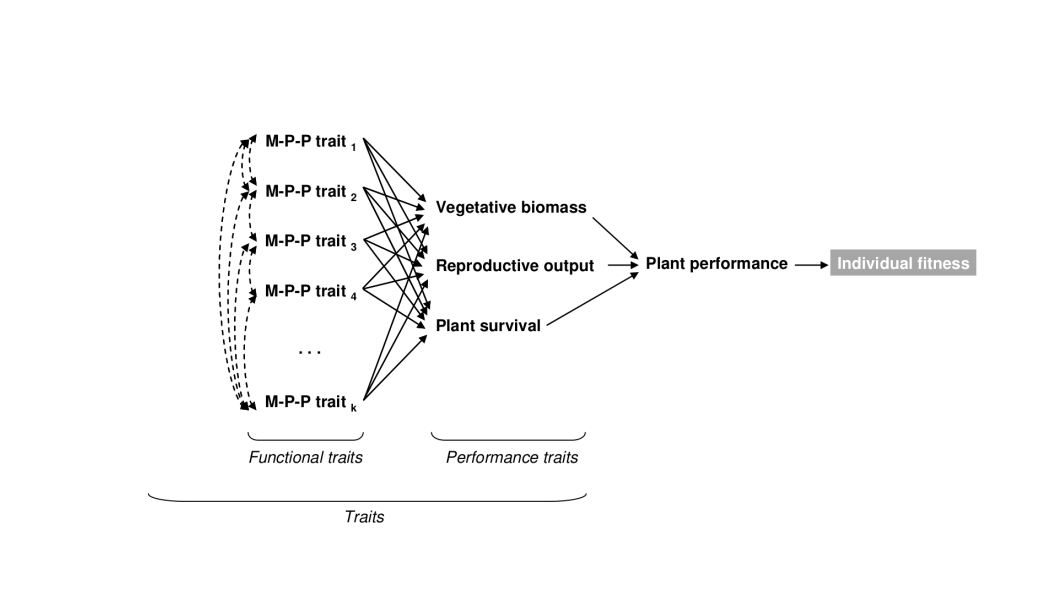
\includegraphics{figures/Violle2007.jpg}
- Mention here the interesting summer school: \url{http://www.cef-cfr.ca/index.php?n=MEmbres.AlisonMunsonPlantTraits?userlang=en}
- List of reference papers in the link above
- 3 types of traits: dynamic, response \& constant, that are linked to the processes we studied in the previous chapter (slow/fast processes)

\hypertarget{representing-400-000-plant-species-in-a-single-model-the-plant-functional-type-approach}{%
\subsection{Representing 400 000 plant species in a single model: the Plant Functional Type approach}\label{representing-400-000-plant-species-in-a-single-model-the-plant-functional-type-approach}}

Short description in UCL 4.3.2\\
No description in Bonan

\begin{itemize}
\tightlist
\item
  Lack of observations for every species
\item
  Computing resources problem (refers to the history of DGVMs from the introduction)
\item
  A simplification based on biome description and plant functionning at the ecosystem level
\item
  Different definitions of PFT: statistical classification, etc.
\item
  Table of classical PFTs used in models here.
\item
  PFT mapping: multi-obs approach based on remote sensing.
\item
  First use of PFTs managed to reproduce well the gradients at the global scale, but now it is unsuficcient.
\end{itemize}

\hypertarget{limits-of-the-pft-representation-in-the-context-of-global-change}{%
\subsection{Limits of the PFT representation in the context of global change}\label{limits-of-the-pft-representation-in-the-context-of-global-change}}

\begin{itemize}
\tightlist
\item
  Including acclimation and adaptation processes
\item
  Dynamic vegetation: Accounting for non-random species turnover
\item
  Quantifying vegetation-environment feedbacks
\item
  Quantifying impacts of biodiversity on ecosytem functioning and climate
\end{itemize}

\hypertarget{from-model-parameters-to-plant-traits}{%
\subsection{From model parameters to plant traits}\label{from-model-parameters-to-plant-traits}}

\begin{itemize}
\tightlist
\item
  Reconciliating modelling with functional ecology.
\item
  Existing databases (TRY)
\item
  Empirical approach: More PFTs with traits instead of model-specific parameters, trait-trait, trait-environment relationships
\item
  Trade-offs: modeling plant strategies --\textgreater{} LES, PES, RES, all the ES :D
\item
  Role of data assimilation in regions without data and to assess spatial variability of vegetation properties
\item
  But: requires lots of observations in space and time.
\end{itemize}

\hypertarget{eco-evolutive-optimality-approaches}{%
\subsection{Eco-evolutive optimality approaches}\label{eco-evolutive-optimality-approaches}}

\begin{itemize}
\tightlist
\item
  New generation of models
\item
  PPA, coordination, ect\ldots{}
\item
  Paper from Oskar.
\end{itemize}

\hypertarget{competition-models}{%
\section{Competition models}\label{competition-models}}

Not in Bonan nor UCL\\
In Bonan Chapter 19 on demography, gap models, etc\ldots{} which is a part of competition.

\hypertarget{representation-of-pfts-in-vegetation-models}{%
\subsection{Representation of PFTs in vegetation models}\label{representation-of-pfts-in-vegetation-models}}

\begin{itemize}
\tightlist
\item
  Parameterization and calibration of PFTs--\textgreater{} data assimilation, traits, model-specific parameters
\item
  representation by pixels
\item
  shared processes, different processes
\item
  interaction between PFTs
\item
  Depend on the model: individual/cohort/big leaf
\end{itemize}

\hypertarget{competition-for-ressources-plant-strategy}{%
\subsection{Competition for ressources / Plant strategy?}\label{competition-for-ressources-plant-strategy}}

\begin{itemize}
\tightlist
\item
  In fact we can extend the trait based approach and plant strategy (PES, etc)
  in the competition and community section?
\item
  Mortality, turnover, etc..
\end{itemize}

\hypertarget{representation-of-trait-distributions}{%
\subsection{Representation of trait distributions}\label{representation-of-trait-distributions}}

\begin{itemize}
\tightlist
\item
  Trade-offs
\end{itemize}

\hypertarget{communities}{%
\section{Communities}\label{communities}}

\begin{itemize}
\tightlist
\item
  Successions and impact on cycles, species composition etc.
\end{itemize}

\hypertarget{what-about-crops}{%
\section{What about crops?}\label{what-about-crops}}

\begin{itemize}
\tightlist
\item
  Not our focus but we don't forget it. A few words to say that specific crop models exists
\item
  Diversity is not a problem anymore
\item
  Plant functional traits are still central to crop modelling, but competition and diversity are no more an issue.
\item
  Other problematics specific to agriculture, such as agro-ecosystems where we have multi layers of vegetation (Trees over crops) --\textgreater{} Very interesting modelling problem and application especially in arid/semi-arid and tropical regions
\end{itemize}

\hypertarget{modelling-vegetation-dynamics-and-demography}{%
\chapter{Modelling vegetation dynamics and demography}\label{modelling-vegetation-dynamics-and-demography}}

\chaptermark{Dynamics}

Bonan Chapter 19.2
Another class of models, known as individual plant or ecosystem demography models, retains the complexity of individual plants or cohorts of similar plants. In these models, ecosystem properties such as carbon storage are the outcome of demographic processes.

\begin{itemize}
\tightlist
\item
  plant populations
\item
  community composition
\item
  ecosystem structure
\item
  driven by demographic processes of recruitment, establishment, growth, and mortality
\end{itemize}

\hypertarget{gap-models-individual-and-cohort-based-models}{%
\section{Gap models, individual and cohort based models}\label{gap-models-individual-and-cohort-based-models}}

\begin{itemize}
\item
  small scale models; landscape represented as a mosaic of hundreds of independent forest patches, each of which can differ in species composition and stage of development in response to disturbance that creates an opening in the canopy
\item
  models track the establishment, growth, and death of individual trees in an area of land.
\item
  Each tree is characterized by its species, stem diameter, height, and age.
\item
  trees compete for light, soil moisture, and nutrients.
\item
  patch undergoes temporal changes in the density, size, and composition of trees with the formation of a gap in the canopy
\item
  Community composition, biomass, productivity, and biogeochemical cycles are emergent outcomes of individual trees interacting among themselves and with the environment to acquire the resources necessary for growth and survival
\item
  cohort-based models define patches based on age since disturbance and simulate the dynamics of cohorts of similar plant functional types rather than tracking every individual.
\item
  Common to each model is the representation of vegetation demography, with age- and size-dependent growth and mortality and in which growth is constrained by allometric relationships of stem diameter with height, sapwood area, leaf area, and biomass. cohort models --\textgreater{} modelling size distributions
\end{itemize}

\hypertarget{allometric-relationships}{%
\section{Allometric relationships}\label{allometric-relationships}}

\begin{itemize}
\tightlist
\item
  link with growth modelling of previuous chapter
\item
  allometric relationships are a critical driver of individual tree growth.
\item
  Height is important for its effect on stem diameter increment, both directly through tree volume growth and indirectly through shading.
\item
  Biomass allocation: empirical equations that constrain foliage, stem, and root mass for a given size tree
\item
  relationship between stem diameter and leaf area drives light extinction in the canopy
\item
  annual growth of a tree is calculated from its diameter and height as modified by light, climate, and site conditions. Growth curves figure 19.5
\end{itemize}

\hypertarget{competition-for-light}{%
\section{Competition for light}\label{competition-for-light}}

\begin{itemize}
\tightlist
\item
  critical driver of forest dynamics
\item
  shading of smaller individuals by taller trees
\item
  vertical profile of leaf area in the patch (vertical structure in which trees are arranged into canopy layers)
\item
  height of a tree determines its location in the cumulative leaf area profile
\item
  light extinction coefficient
\item
  figure 19.6: representation of plant canopies
\end{itemize}

\hypertarget{seed-dispersal-and-recruitment}{%
\section{Seed dispersal and recruitment}\label{seed-dispersal-and-recruitment}}

\begin{itemize}
\item
  regeneration: stochastic process
\item
  seeds of species are assumed to be present on-site
\item
  available light at the forest floor, climate tolerances, and other site conditions determine which species become established.
\item
  sprouting based on size
\item
  Species are characterized by life history characteristics + maybe add example of herb layer models of FORNALAB
\end{itemize}

\hypertarget{mortality}{%
\section{Mortality}\label{mortality}}

\begin{itemize}
\item
  stochastic process
\item
  Trees die with a constant probability each year
\item
  The probability of mortality increases when tree growth is less than some minimum
\item
  disturbance related mortality : Wildfire and insect outbreaks can be included
\item
  The occurrence of fire is treated stochastically with an annual probability of burning. An individual patch may, for example, have a 1\% change of burning in any given year.
\end{itemize}

\hypertarget{part-upscaling-and-applications}{%
\part{Upscaling and applications}\label{part-upscaling-and-applications}}

\hypertarget{spatial-heterogeneity-landscape-scale-metapopulations}{%
\chapter{Spatial heterogeneity, landscape scale, metapopulations}\label{spatial-heterogeneity-landscape-scale-metapopulations}}

\chaptermark{Heterogeneity}

\hypertarget{patch-dynamics}{%
\section{Patch dynamics}\label{patch-dynamics}}

Some references:
- Book: The ecology of natual disturance and patch dynamics, Pickett \& White, 2013

\hypertarget{spatial-heterogeneity-definitions}{%
\subsection{Spatial heterogeneity: Definitions}\label{spatial-heterogeneity-definitions}}

\begin{itemize}
\tightlist
\item
  Definition of Patch Dynamics, Perturbation, Disturbance:
\item
  Spatial heterogeneity
\item
  Resilience and shifts
\end{itemize}

\hypertarget{impact-of-heterogeneity-on-ecosystem-fonctionning-and-environmental-feedbacks}{%
\subsection{Impact of heterogeneity on ecosystem fonctionning and environmental feedbacks}\label{impact-of-heterogeneity-on-ecosystem-fonctionning-and-environmental-feedbacks}}

\begin{itemize}
\tightlist
\item
  Show examples here of the impact of heterogeneity
\item
  Application in the design of nature reserves for example
\end{itemize}

\hypertarget{heterogeneity-is-a-matter-of-resolution}{%
\subsection{Heterogeneity is a matter of resolution}\label{heterogeneity-is-a-matter-of-resolution}}

\begin{itemize}
\tightlist
\item
  Imbricated levels of heterogeneity depending on spatial and temporal resolution
\item
  Heterogeneity is also a matter of the studied question: important in term of modelling since it will govern how processes are implemented
\end{itemize}

\hypertarget{representation-in-vegetation-models-what-are-the-drivers-of-spatial-heterogeneity}{%
\subsection{Representation in Vegetation models: what are the drivers of spatial heterogeneity?}\label{representation-in-vegetation-models-what-are-the-drivers-of-spatial-heterogeneity}}

\begin{itemize}
\tightlist
\item
  List here the different drivers
\item
  Heterogeneity is a patchwork of homogeneity in most models
\item
  But we can still represent dynamics in heterogeneity --\textgreater{} mortality, growth and shifts in species composition
\end{itemize}

\hypertarget{disturbances-and-patch-dynamics}{%
\subsection{Disturbances and Patch dynamics}\label{disturbances-and-patch-dynamics}}

\begin{itemize}
\tightlist
\item
  We listed the different drivers above, we will now discuss in detail the most important aspects affecting patch dynamics
\item
  Link to land-use and disturbance
\end{itemize}

\hypertarget{land-use-changes}{%
\section{Land-use changes}\label{land-use-changes}}

\begin{itemize}
\tightlist
\item
  Land use is linked to spatial heterogeneity and patch dynamics
\end{itemize}

\hypertarget{role-of-land-use-in-global-emissions-and-biogeochemicel-cycles}{%
\subsection{Role of Land-use in global emissions and biogeochemicel cycles}\label{role-of-land-use-in-global-emissions-and-biogeochemicel-cycles}}

\begin{itemize}
\tightlist
\item
  impact C stocks and fluxes
\item
  impact on nutrients (depletion over rotations, etc\ldots)
\item
  important impact on respiration
\item
  vegetation cover and biophysical impact: albedo, etc\ldots{}
\item
  Specific case of deforestation, one of the most important imapct (make a paragraph on that?)
\item
  How are fluxes attributed to land use in gas emission assessments? --\textgreater{} central role of vegetation modeling
\end{itemize}

\hypertarget{the-important-role-of-land-use-in-the-water-cycle}{%
\subsection{The important role of land use in the water cycle}\label{the-important-role-of-land-use-in-the-water-cycle}}

\begin{itemize}
\tightlist
\item
  Affects regional precipitations
\item
  Affects water routing
  --\textgreater{} Compared to the local impact on vegetation, here we touch something that will have an impact for the surrounding regions
\end{itemize}

\hypertarget{monitoring-land-use}{%
\subsection{Monitoring land-use}\label{monitoring-land-use}}

\begin{itemize}
\tightlist
\item
  remote sensing, rapid link to other courses
\end{itemize}

\hypertarget{how-land-use-is-represented-in-vegetation-models}{%
\subsection{How Land-use is represented in vegetation models?}\label{how-land-use-is-represented-in-vegetation-models}}

\begin{itemize}
\tightlist
\item
  Compared to vegetation dynamic which is process-based, here land use is imposed.
\item
  management
\item
  urban areas
\end{itemize}

\hypertarget{natural-and-anthropogenic-disturbances}{%
\section{Natural and Anthropogenic disturbances}\label{natural-and-anthropogenic-disturbances}}

\begin{itemize}
\tightlist
\item
  We provide an overview of disturbances but we will detail only one of each: Fires and Management
\end{itemize}

\hypertarget{wind-and-extrem-events}{%
\subsection{Wind and extrem events}\label{wind-and-extrem-events}}

\begin{itemize}
\tightlist
\item
  Modelling storms
\item
  Modelling heat and cold waves, frost impact
\end{itemize}

\hypertarget{herbivory}{%
\subsection{Herbivory}\label{herbivory}}

\begin{itemize}
\tightlist
\item
  Yes herbivory is represented in vegetation models :D
\item
  Palability traits/ fixed fraction/ insects
\end{itemize}

\hypertarget{modelling-fires}{%
\subsection{Modelling fires}\label{modelling-fires}}

\begin{itemize}
\tightlist
\item
  In UCL Practical chap.~6
\item
  For estimating the impact on ecosystems
\item
  To be able to predict fires
\item
  Observation of fires and quantifications of fluxes
\item
  Fires and deposition
\item
  Aerosols
\item
  Modelling ``fire'' traits, drought and temperature stress in models to simulate fires
\end{itemize}

\hypertarget{human-activity-management-and-urban-areas}{%
\subsection{Human activity: Management and urban areas}\label{human-activity-management-and-urban-areas}}

\begin{itemize}
\tightlist
\item
  Forest management: existing models, representation of forestry and use of models
\item
  Fertilization and irrigation in vegetation models
\item
  Urban areas in vegetation models
\item
  Concrete application: Paper of Luyssaert: forest management in Europe did not help in mitigating climate change.
\end{itemize}

\hypertarget{the-specific-case-of-co2-and-temperature-increase}{%
\subsection{The specific case of CO2 and temperature increase}\label{the-specific-case-of-co2-and-temperature-increase}}

\begin{itemize}
\tightlist
\item
  conclude the chapter here by refering to climate change, one of the biggest ``Continuous'' distrubance compared to previous ``discrete'' disturbances
\item
  Simulating acclimation and adaptation
\item
  refers to chapter 2 for acclimation of processes
\item
  refers to chapter 11 for scenarios
\end{itemize}

\hypertarget{upscaling-from-the-leaf-to-the-globe}{%
\chapter{Upscaling from the leaf to the globe}\label{upscaling-from-the-leaf-to-the-globe}}

\chaptermark{Globe}

Some references:
- Scalling processes and problems, Jarvis 1995
- upscalling in global change research, Harvey 2000

\hypertarget{spatial-and-temporal-non-linearities-cascading-effect-in-the-earth-system}{%
\section{Spatial and temporal non-linearities: Cascading effect in the Earth system}\label{spatial-and-temporal-non-linearities-cascading-effect-in-the-earth-system}}

\begin{itemize}
\tightlist
\item
  spatial upscalling
\item
  temporal upscalling
\item
  classification of upscalling problems:

  \begin{itemize}
  \tightlist
  \item
    Spatial variability + process nonlinearity
  \item
    Minimim scale to observe the process
  \item
    Different processes dominate at different scales
  \item
    Feedbacks between scales
  \item
    Development of emergent properties
  \item
    Edge effects
  \item
    Temporal lag dependent on spatial scale change
  \item
    Collective response with differential effects
  \end{itemize}
\item
  Solutions to upscaling problems:

  \begin{itemize}
  \tightlist
  \item
    Ignore (easy solution)
  \item
    Increase model resolution (now more and more possible thanks to computing ressources, and data assimilation)
  \item
    etc\ldots{} ** Nice review in Harvey 2000 **
  \end{itemize}
\end{itemize}

--\textgreater{} Solution depends on the application, show some examples here

\hypertarget{land-surface-models}{%
\section{Land surface models}\label{land-surface-models}}

\begin{itemize}
\tightlist
\item
  Dependence to other disciplines (Biology, ecology, physics, chemistry (VOC, etc), hydrology, pedology, datascience and mathematics, etc\ldots)
\item
  Figure 1.7 from Bonan
\item
  UCL 4.2: Land surface schemes
\item
  Focus on the coupling of different models and what it implies, not the technical aspects
  \#\#\# Soil-Vegetation-Atmosphere-Transer models
\item
  Description of SVAT models, regroups what we studied in Chap1-9
\end{itemize}

\hypertarget{dvgms-as-a-part-of-earth-system-models}{%
\section{DVGMs as a part of Earth System Models}\label{dvgms-as-a-part-of-earth-system-models}}

\begin{itemize}
\tightlist
\item
  Partially in UCL 4.3.3
\end{itemize}

\hypertarget{one-biosphere}{%
\subsection{One Biosphere}\label{one-biosphere}}

\begin{itemize}
\tightlist
\item
  Chapter 1 of Bonan, specifically 1.5
\item
  Coupling to other components
\end{itemize}

\hypertarget{atmosphere-ocean-lakes-and-urban-areas}{%
\subsection{Atmosphere, Ocean, lakes and urban areas}\label{atmosphere-ocean-lakes-and-urban-areas}}

\begin{itemize}
\tightlist
\item
  Rapid desciption of other models
\item
  Reference here to previous chapter on heterogeneity
\end{itemize}

\hypertarget{coupling-of-processes-with-different-time-steps-and-regional-scale}{%
\subsection{Coupling of processes with different time steps and regional scale}\label{coupling-of-processes-with-different-time-steps-and-regional-scale}}

\hypertarget{simulating-feedbacks}{%
\subsection{Simulating feedbacks}\label{simulating-feedbacks}}

\begin{itemize}
\tightlist
\item
  Nice transition to chap 11 with future scenarii
\end{itemize}

\hypertarget{model-projections-and-scenario-analysis}{%
\chapter{Model projections and scenario analysis}\label{model-projections-and-scenario-analysis}}

\chaptermark{Projections}

\hypertarget{climate-scenarios}{%
\section{Climate scenarios}\label{climate-scenarios}}

\hypertarget{representative-concentration-pathway-rcp-scenarios}{%
\subsection{Representative Concentration Pathway (RCP scenarios)}\label{representative-concentration-pathway-rcp-scenarios}}

\begin{itemize}
\tightlist
\item
  How scenarios are defined
\item
  How current emissions are measured and attributed to different factors?
\end{itemize}

\hypertarget{different-models-different-rcp}{%
\subsection{Different models, different RCP}\label{different-models-different-rcp}}

\begin{itemize}
\tightlist
\item
  The central role of ESM: coupling to Atmosphere and Ocean and feedbacks
\item
  Here refers to preivous Chapter 10
\item
  list some examples and differences: IPSL, HadGEM, etc\ldots{}
\end{itemize}

\hypertarget{use-of-rcp-in-vegetation-modelling}{%
\subsection{Use of RCP in vegetation modelling}\label{use-of-rcp-in-vegetation-modelling}}

\begin{itemize}
\tightlist
\item
  ENSEMBLE simulations
\item
  IPCC
\item
  Example of applications
\end{itemize}

\hypertarget{how-can-we-evaluate-future-scenarios}{%
\subsection{How can we evaluate future scenarios?}\label{how-can-we-evaluate-future-scenarios}}

\begin{itemize}
\tightlist
\item
  FACE
\item
  Rainfall exclusion experiments
\item
  Natural gradient (Iceland and soil temperature based on volcano and geothermy)
\end{itemize}

\hypertarget{the-central-role-of-paleo-studies-and-historical-datasets.}{%
\subsection{The central role of Paleo studies and historical datasets.}\label{the-central-role-of-paleo-studies-and-historical-datasets.}}

\begin{itemize}
\tightlist
\item
  Good performance for past and current conditions is mandatory to evaluate future scenarios
\item
  Here remind the central role of experiments and monitoring
\end{itemize}

\hypertarget{land-use-scenarios}{%
\section{Land-use scenarios}\label{land-use-scenarios}}

\hypertarget{construction-of-land-use-scenarios}{%
\subsection{Construction of Land-use scenarios}\label{construction-of-land-use-scenarios}}

\begin{itemize}
\tightlist
\item
  Hyde for historical land-use, \url{https://themasites.pbl.nl/tridion/en/themasites/hyde/}
\item
  Scenario for future land-use
\end{itemize}

--\textgreater{} We can follow the same structure as for RCP?

\hypertarget{how-can-we-evaluate-land-use-scenarios}{%
\subsection{How can we evaluate land use scenarios?}\label{how-can-we-evaluate-land-use-scenarios}}

\begin{itemize}
\tightlist
\item
  Based on historical data
\item
  Remote sensing
\end{itemize}

\hypertarget{management-scenarios}{%
\section{Management scenarios}\label{management-scenarios}}

\hypertarget{construction-of-land-use-scenarios-1}{%
\subsection{Construction of Land-use scenarios}\label{construction-of-land-use-scenarios-1}}

\hypertarget{how-can-we-evaluate-management-scenarios}{%
\subsection{How can we evaluate management scenarios?}\label{how-can-we-evaluate-management-scenarios}}

\hypertarget{some-concrete-applications-of-vegetation-models}{%
\section{Some concrete applications of vegetation models}\label{some-concrete-applications-of-vegetation-models}}

\begin{itemize}
\tightlist
\item
  As a conclusion of the whole course I see a nice diagram that we constructed throughout the course with small boxes added to each others and we link that to all the possible application
\end{itemize}

\hypertarget{part-appendix}{%
\part{Appendix}\label{part-appendix}}

\hypertarget{contributing-to-this-document}{%
\chapter*{Contributing to this document}\label{contributing-to-this-document}}
\addcontentsline{toc}{chapter}{Contributing to this document}

\hypertarget{first-steps}{%
\section*{First steps}\label{first-steps}}
\addcontentsline{toc}{section}{First steps}

First, visit the course webpage on \url{https://github.com/femeunier/VegMod_course}, and fork it to your own github account. Open a RStudio session and (if it is your first time with git) introduce yourself:

\begin{Shaded}
\begin{Highlighting}[]
\FunctionTok{git}\NormalTok{ config {-}{-}global user.name }\StringTok{"FULLNAME"}
\FunctionTok{git}\NormalTok{ config {-}{-}global user.email you@yourdomain.example.com}
\end{Highlighting}
\end{Shaded}

Note that you can do every single step below using the terminal and the git tabs in RStudio. Clone the newly forked folder to your local machine:

\begin{Shaded}
\begin{Highlighting}[]
\FunctionTok{git}\NormalTok{ clone https://github.com/femeunier/VegMod\_course.git}
\end{Highlighting}
\end{Shaded}

or using SSH (to set up it first, see for instance \url{https://help.github.com/en/github/authenticating-to-github/connecting-to-github-with-ssh})

\begin{Shaded}
\begin{Highlighting}[]
\FunctionTok{git}\NormalTok{ clone git@github.com:femeunier/VegMod\_course.git}
\end{Highlighting}
\end{Shaded}

Define upstream

\begin{Shaded}
\begin{Highlighting}[]
\BuiltInTok{cd}\NormalTok{ VegMod\_course}
\FunctionTok{git}\NormalTok{ remote add upstream git@github.com:femeunier/VegMod\_course.git}
\end{Highlighting}
\end{Shaded}

\hypertarget{new-pull-request}{%
\section*{New pull request}\label{new-pull-request}}
\addcontentsline{toc}{section}{New pull request}

Get the latest code from the main repository

\begin{Shaded}
\begin{Highlighting}[]
\FunctionTok{git}\NormalTok{ pull upstream master}
\end{Highlighting}
\end{Shaded}

Create a new branch (here new\_branch is the new branch's name)

\begin{Shaded}
\begin{Highlighting}[]
\FunctionTok{git}\NormalTok{ checkout {-}b new\_branch}
\end{Highlighting}
\end{Shaded}

Do some coding, add files and commit them

\begin{Shaded}
\begin{Highlighting}[]
\FunctionTok{git}\NormalTok{ add filepath}
\FunctionTok{git}\NormalTok{ commit {-}m “Message”}
\end{Highlighting}
\end{Shaded}

Push your changes to your github (when a feature is working, a set of bugs are fixed, or you need to share progress with others).

\begin{Shaded}
\begin{Highlighting}[]
\FunctionTok{git}\NormalTok{ push origin new\_branch}
\end{Highlighting}
\end{Shaded}

Before submitting code back to the main repository, make sure that book compiles (buikd book). Open the PR online by visiting your github repository. To ease those previous steps you can take advantage of the git GUI in RStudio. To do so, create a new project from an existing directory.

\hypertarget{supporting-material}{%
\chapter*{Supporting material}\label{supporting-material}}
\addcontentsline{toc}{chapter}{Supporting material}

Crash course, basic programming (R), theory about model evaluation etc.

\hypertarget{part-practicals}{%
\part{Practicals}\label{part-practicals}}

\hypertarget{practical-a}{%
\chapter*{Practical A}\label{practical-a}}
\addcontentsline{toc}{chapter}{Practical A}

PC-room, supervised exercise

Simple model on diurnal variation in solar angle, radiation extinction and photosynthesis in vegetation types with different and canopy structure and LAI: grassland, broadleaved forest, coniferous forest

Scale: aggregated stand level (big leaf model)

Methodological focus: model formulation: translating a few equations into code

Methodological focus: compiling code, running model, reading input-output

\hypertarget{practical-b}{%
\chapter*{Practical B}\label{practical-b}}
\addcontentsline{toc}{chapter}{Practical B}

Group work, report, PC room

Modelling diurnal cycle of carbon and water fluxes for flux tower sites (Savanna's Sahel)

Scale: aggregated stand level

Methodological focus: model-data comparison (goodness-of-fit), simple parameter optimisation

\hypertarget{practical-c}{%
\chapter*{Practical C}\label{practical-c}}
\addcontentsline{toc}{chapter}{Practical C}

PC-room, supervised exercise

Modelling the size structure of a temperate forest (stand diameter distribution)

Scale: forest stand

Methodological focus: initial conditions

\hypertarget{practical-d}{%
\chapter*{Practical D}\label{practical-d}}
\addcontentsline{toc}{chapter}{Practical D}

Group work, report, PC room

Modelling carbon stocks (above and belowground) and fluxes

Scale: ecosystem

Methodological focus: Spinup and sensitivity analysis (testing which climate variables have strongest impact on stocks)

\hypertarget{practical-e}{%
\chapter*{Practical E}\label{practical-e}}
\addcontentsline{toc}{chapter}{Practical E}

PC-room, supervised exercise

Simulating forest succession, meta-analysis of trait dataset to prescribe vegetation functional composition (using PEcAn-framework)

Scale: landscape

Methodological focus: parameter meta-analysis (PFT construction), data assimilation

\hypertarget{practical-f}{%
\chapter*{Practical F}\label{practical-f}}
\addcontentsline{toc}{chapter}{Practical F}

PC-room, group work, microteaching

Climate/land use/management scenario analysis

Scale: site/globe? (Pecan framework) each group choses a question and a model

Methodological focus: sensitivity and uncertainty analysis

  \bibliography{book.bib,packages.bib}

\end{document}
